
\chapter{Corrélations quantiques}

\minitoc

\bigskip

Nos incursions dans le monde quantique ce sont jusqu'à présent limités aux états
à un quanton. L'objet de ce chapitre est la description d'états à deux quantons
qui conduisent à des configurations très riches dites \textbf{intriquées} ou
\textbf{corrélées}. Ces corrélations sont à la base du calcul quantique. Une
fois assimilé le cas à deux quantons, la généralisation à un nombre quelconque
de quantons est facile.

Dans la vie courante, on a par exemple des \emph{corrélations par échange du
signal} tel que le feu rouge correspond à l'arrêt des véhicules et au passage
des piétons. Mais on a pas de corrélation entre particules classiques.

Le chapitre commence avec la \textbf{section \ref{sec:ProdTen}} qui introduit
les notions de produit tensoriel et d'états intriqués indispensables à la
description des états à plusieurs quantons. La \textbf{section \ref{sec:Bell}}
est consacrée à l'étude des importantes conséquences physiques telles les
inégalités de Bell et les interférences des états corrélés, qui permettent de
mettre en exergue le caractère non local et non séparable de la théorie
quantique. En effet, il apparaît que
\begin{enumerate}
\item les corrélations quantiques ne disparaissent pas lorsqu'on augmente la
distance entre les quantons, et leur origine ne peut être la réception d'un
signal commun;

\item les corrélations quantiques violent les inégalités de Bell et donc leur
origine ne peut non plus être une décision commune prise à la source.
\end{enumerate}

La dernière section, \textbf{section \ref{sec:IQ}}, est réservée aux
applications en information quantique comme la cryptographie et la téléportation
quantique.

\section{Produit tensoriel et états intriqués}
\label{sec:ProdTen}

\subsection{États}

Soient deux systèmes physiques isolés $(S_{1})$ et $(S_{2})$, d'espaces d'états
correspondants respectifs $\mathcal{H}_{1}$ et $\mathcal{H}_{2}$. Si on
considère l'ensemble de ces deux états comme un système unique $(S)$, quel est
l'espace des états $\mathcal{H}$ associé?

\colorbox[gray]{0.8}{
\parbox[c]{0.9\textwidth}{
\begin{definition}
Par définition, l'espace d'états $\mathcal{H}$ est appelé \textbf{produit
tensoriel} de $\mathcal{H}_{1}$ et $\mathcal{H}_{2}$, et noté $\mathcal{H}%
=\mathcal{H}_{1}\otimes\mathcal{H}_{2}$, si à tout couple de vecteurs,
$(\ket{\psi_{1}},\ket{\psi_{2}})\in\mathcal{H}_{1}\times\mathcal{H}_{2}$, on
associe un vecteur de $\mathcal{H}$, noté $\ket{\psi_{1}}\otimes\ket{\psi_{2}}$
et appelé produit tensoriel de $\ket{\psi_{1}}$ et $\ket{\psi_{2}}$, tel que
cette correspondance soit linéaire par rapport à la multiplication par des
scalaires, et distributive par rapport à l'addition vectorielle:
\begin{subequations}%
\begin{align}
[\ket{\psi_{1}}+\lambda\ket{\psi_{1}^{\prime}}]\otimes\ket{\psi_{2}} &
=\ket{\psi_{1}}\otimes\ket{\psi_{2}}+\lambda\ket{\psi_{1}^{\prime}}\otimes
\ket{\psi_{2}},\\
\ket{\psi_{1}}\otimes[\ket{\psi_{2}}+\lambda\ket{\psi_{2}^{\prime}}]   &
=\ket{\psi_{1}}\otimes\ket{\psi_{2}}+\lambda\ket{\psi_{1}}\otimes\ket{\psi_{2}^{
\prime}},
\end{align}
\end{subequations}%
et tel que si $\{\ket{\psi_{1}^{i}}\}$ et $\{\ket{\psi_{2}^{j}}\}$ sont
respectivement des bases de $\mathcal{H}_{1}$ et $\mathcal{H}_{2}$, alors
$\{\ket{\psi_{1}^{i}}\otimes\ket{\psi_{2}^{j}}\}$ est une base de
$\mathcal{H}$.
\end{definition}
}}
\medskip

Pour des raisons de simplicité, on note le plus souvent
\begin{equation}
\ket{\psi_{1}}\otimes\ket{\psi_{2}}=\ket{\psi_{1}}\ket{\psi_{2}}
=\ket{\psi_{1}\psi_{2}}.
\end{equation}

\colorbox[gray]{0.8}{
\parbox[c]{0.9\textwidth}{
\begin{definition}
Le \textbf{produit scalaire} sur $\mathcal{H}=\mathcal{H}_{1}\otimes
\mathcal{H}_{2}$ se définit de la manière suivante%
\begin{equation}
\langle\psi_{1}^{\prime}\psi_{2}^{\prime}\ket{\psi_{1}\psi_{2}}=
\langle\psi_{1}^{\prime}\ket{\psi_{1}}
\langle\psi_{2}^{\prime}\ket{\psi_{2}}.
\end{equation}
\end{definition}
}}
\medskip

Si $\{\ket{n}\}$ est une base orthonormée de $\mathcal{H}_{1}$ et $\{\ket{m}\}$
une base orthonormée de $\mathcal{H}_{2}$ telles que%
\begin{equation}
\ket{\psi_{1}}=\sum_{n=1}^{N}\alpha_{n}\ket{n},\ \ket{\psi_{2}}=\sum_{m=1}^{M}
\alpha_{m}\ket{m},
\end{equation}
alors%
\begin{equation}
\ket{\psi_{1}\psi_{2}}=\sum_{n,m}\alpha_{n}\alpha_{m}\ket{nm},
\label{eq:PT2}%
\end{equation}
avec%
\begin{equation}
\langle n^{\prime}m^{\prime}\ket{nm}=\delta_{n^{\prime}n}\delta_{m^{\prime}m}.
\end{equation}

\begin{example}\label{expl:tensoEt}
On considère dans la base $\{\ket{0},\ket{1}\}$ les vecteurs d'état
$\ket{\psi_1}=\frac{1}{\sqrt{2}}(\ket{0}-\ket{1})=
\frac{1}{\sqrt{2}}\binom{1}{-1}$ et
$\ket{\psi_{2}}=\frac{1}{\sqrt{2}}(\ket{0}+\ket{1})=\frac{1}{\sqrt{2}}
\binom{1}{1}$. Dans la base $\{\ket{00},\ket{01},\ket{10},\ket{11}\}$ le produit
tensoriel $\ket{\psi_{1}}\otimes\ket{\psi_{2}}$ a pour matrice%
\begin{equation}
\ket{\psi_{1}}\otimes\ket{\psi_{2}}=\frac{1}{\sqrt{2}}\binom{1.\ket{\psi_{2}}}{
-1.\ket{\psi_{2}}}=\frac{1}{2}\begin{pmatrix}
1\\
1\\
-1\\
-1
\end{pmatrix}.
\end{equation}

\end{example}

On peut considérer qu'un état produit $\ket{\psi_{1}} \otimes\ket{\psi_{2}}$
représente la simple juxtaposition de deux systèmes, l'un dans l'état
$\ket{\psi_{1}}$ et l'autre dans l'état $\ket{\psi_{2}}$. On dit encore que,
dans un tel état, les deux systèmes sont \textbf{sans corrélations}: les
résultats de deux types de mesures pourtant soit sur un système, soit sur
l'autre, correspondent à des variables aléatoires indépendantes. Une telle
situation est réalisée lorsque les deux systèmes ont été préparés indépendamment
et séparément dans les états $\ket{\psi_{1}}$ et $\ket{\psi_{2}}$ et qu'on les
réunit ensuite, sans qu'ils interagissent.

\subsection{Opérateurs}

Soient $A$ et $B$ deux opérateurs agissant respectivement dans $\mathcal{H}_{1}$
et $\mathcal{H}_{2}$. On peut construire un opérateur $A\otimes B$ agissant dans
$\mathcal{H}=\mathcal{H}_{1}\otimes\mathcal{H}_{2}$ tel que%
\begin{equation}
(A\otimes B)\ket{\psi_{1}\psi_{2}}=A\ket{\psi_{1}}\otimes B\ket{\psi_{2}}.
\end{equation}
Si $A$ et $B$ sont des opérateurs hermitiens, alors $A\otimes B$ est un
opérateur hermitien.

Une classe simple des opérateurs de $\mathcal{H}$ est
\begin{equation}
A\otimes\mathbb{I}_{B}\text{ et }\mathbb{I}_{A}\otimes B.
\end{equation}
Il est à noter que
\begin{equation}
(A\otimes B)\cdot(C\otimes D)=(AC)\otimes(BD).
\end{equation}
Ainsi%
\begin{equation}
[A\otimes\mathbb{I}_{B},\mathbb{I}_{A}\otimes B]=(A\otimes\mathbb{I}_{B})\cdot
(\mathbb{I}_{A}\otimes B)-(\mathbb{I}_{A}\otimes B)\cdot(A\otimes\mathbb{I}_{B})
=0.
\end{equation}

Si $\ket{\psi_{1}}$ est un vecteur propre de l'opérateur $A$ avec la valeur
propre $a$, $A\ket{\psi_{1}}=a\ket{\psi_{1}}$, alors $\ket{\psi_{1}\otimes
\psi_{2}}$ est aussi vecteur propre de $A\otimes\mathbb{I}_{B}$ avec la valeur
propre $a$:%
\begin{equation}
A\otimes\mathbb{I}_{B}\ket{\psi_{1}\otimes\psi_{2}}=a\ket{\psi_{1}\otimes\psi_{2
}}.
\end{equation}
On omet très souvent d'écrire explicitement les opérateurs identités
$\mathbb{I}_{A}$ et $\mathbb{I}_{B}$ pour écrire simplement%
\begin{subequations}%
\begin{equation}
A\ket{\psi_{1}\otimes\psi_{2}}=a\ket{\psi_{1}\otimes\psi_{2}},
\end{equation}
ou
\begin{equation}
A\ket{\psi_{1}\psi_{2}}=a\ket{\psi_{1}\psi_{2}},
\end{equation}%
\end{subequations}%
en supprimant le produit tensoriel.

\begin{example}\label{expl:tensoOp}
La matrice représentant le produit tensoriel des matrices de Pauli $\sigma
_{x}=\begin{pmatrix}
0 & 1\\
1 & 0
\end{pmatrix}$ et $\sigma_{z}=\begin{pmatrix}
1 & 0\\
0 & -1
\end{pmatrix}$ est%
\begin{equation}
\sigma_{x}\otimes\sigma_{z}=\begin{pmatrix}
0.\sigma_{z} & 1.\sigma_{z}\\
1.\sigma_{z} & 0.\sigma_{z}
\end{pmatrix}
=\begin{pmatrix}
0 & 0 & 1 & 0\\
0 & 0 & 0 & -1\\
1 & 0 & 0 & 0\\
0 & -1 & 0 & 0
\end{pmatrix}.
\end{equation}

\end{example}

\begin{exercise}
 Évaluer $\sigma_{z}\otimes\sigma_{x}$ et conclure.
\end{exercise}
\begin{exercise}
 Suppose that $A$ is a projector in $\mathcal{H}_{1}$ where $A=\ket{0}\bra{0}$
and $B$ is a projector in $\mathcal{H}_{2}$ where $B=\ket{1}\bra{1}$. Find
\begin{equation}
 A\otimes B\left( \frac{\ket{01}+\ket{10}}{\sqrt{2}}\right)
\end{equation}
\end{exercise}
\begin{footnotesize}
\begin{solution}
\begin{equation}
 \begin{split}
A\otimes B\left( \frac{\ket{01}+\ket{10}}{\sqrt{2}}\right) & =
\frac{1}{\sqrt{2}}[\ket{A0}\ket{B1}+\ket{A1}\ket{B0}]\\
& =\frac{1}{\sqrt{2}}[\ket{0}\bra{0}0\rangle\ket{1}\bra{1}1\rangle+\ket{0}\bra
{0}1\rangle\ket{1}\bra{1}0\rangle]=\frac{1}{\sqrt{2}}\ket{01}.
\end{split}
\end{equation}
\end{solution}
\end{footnotesize}

\begin{exercise}
 A system is in the state
\begin{equation}
 \ket{\psi}=\frac{1}{\sqrt{8}}\ket{00}+\sqrt{\frac{3}{8}}\ket{01}+\frac{1}{2}
\ket{10}+\frac{1}{2}\ket{11}
\end{equation}
\begin{enumerate}
 \item What is the probability that measurement finds the system in the state
$\ket{\phi}=\ket{01}$?
\item What is the probability that measurement finds the first qubit in the
state $\ket{0}$? What is the state of the system after measurement?
\end{enumerate}
\end{exercise}

\begin{footnotesize}
\begin{solution}
\begin{enumerate}
 \item Given that the system is in the state $\ket{\psi}$, the probability of
finding it in the state $\ket{\phi}=\ket{01}$ is calculated using the Born
rule, which is $\mathcal{P} = |\langle\phi\ket{\psi}|^2$. Since $\langle
0\ket{1} = \langle 1\ket{0}=0$, we have
\begin{equation}
\begin{split}
 \langle\phi\ket{\psi} & = \bra{01}\left(\frac{1}{\sqrt{8}}\ket{00}+
\sqrt{\frac{3}{8}}\ket{01}+\frac{1}{2}\ket{10}+\frac{1}{2}\ket{11}\right)\\
 & =\sqrt{\frac{3}{8}}\langle0\ket{0}\langle1\ket{1}=\sqrt{\frac{3}{8}}.
\end{split}
\end{equation}
Therefore the probability is
\begin{equation}
 \mathcal{P}=|\langle\phi\ket{\psi}|^2=\frac{3}{8}.
\end{equation}
\item To find the probability that measurement finds the first qubit in the
state $\ket{0}$, we can apply $P_0\otimes\mathbb{I}=\ket{0}\bra{0}\otimes
\mathbb{I}$ to the state. So the projection operator $P_0$ is applied to the
first qubit and the identity operator to the second qubit, leaving the second
qubit unchanged.

This obtains
\begin{equation}
 \begin{split}
P_0\otimes\mathbb{I}\ket{\psi} & =\ket{0}\bra{0}\otimes\mathbb{I}\left(\frac{1}{
\sqrt{8}}\ket{00}+\sqrt{\frac{3}{8}}\ket{01}+\frac{1}{2}\ket{10}+\frac{1}{2}\ket
{11}\right)\\
 & = \frac{1}{\sqrt{8}}\ket{0}\langle0\ket{0}\otimes\ket{0}+\sqrt{\frac{3}{8}}
\ket{0}\langle0\ket{0}\otimes\ket{1}=
\frac{1}{\sqrt{8}}\ket{00}+\sqrt{\frac{3}{8}}\ket{01}
\end{split}
\end{equation}
The probability of obtaining this result is
\begin{equation}
 \begin{split}
\mathcal{P} & =\bra{\psi}P_0\otimes\mathbb{I}\ket{\psi}=
\left(\frac{1}{\sqrt{8}}\bra{00}+\sqrt{\frac{3}{8}}\bra{01}+\frac{1}{2}\bra{10}
+\frac{1}{2}\bra{11}\right)\left(\frac{1}{\sqrt{8}}\ket{00}+\sqrt{\frac{3}{8}}
\ket{01} \right) \\
& = \frac{1}{8}+\frac{3}{8}=\frac{1}{2}.
\end{split}
\end{equation}
The state of the system after measurement using (\ref{eq:PrReduc}) is found to
be
\begin{equation}
 \frac{\frac{1}{\sqrt{8}}\ket{00}+\sqrt{\frac{3}{8}}\ket{01}}{\sqrt{\bra{\psi}
P_0\otimes\mathbb{I}\ket{\psi}}}=\sqrt{2}\left(
\frac{1}{\sqrt{8}}\ket{00}+\sqrt{\frac{3}{8}}\ket{01}\right)=
\frac{1}{2}\ket{00}+\frac{\sqrt{3}}{2}\ket{01}
\end{equation}
\end{enumerate}

\end{solution}
\end{footnotesize}

\subsection{États corrélés ou intriqués}

Soient deux qubits de $\mathcal{H}_{A}$ et $\mathcal{H}_{B}$,
\begin{subequations}
\begin{align}
\ket{\varphi_{A}} & =a_{0}\ket{0_{A}}+a_{1}\ket{1_{A}} ,\ |a_{0}|^{2}+
|a_{1}|^{2}=1,\\
\ket{\varphi_{B}} & =b_{0}\ket{0_{B}}+b_{1}\ket{1_{B}} ,\ |b_{0}|^{2}+
|b_{1}|^{2}=1.
\end{align}%
\end{subequations}%
Le produit tensoriel
$\ket{\varphi_{A}\otimes\varphi_{B}}$ est donné suivant (\ref{eq:PT2}) par
\begin{equation}
\ket{\varphi_{A}\otimes\varphi_{B}}=a_{0}b_{0}\ket{0_{A}\otimes0_{B}}
+a_{0}b_{1}\ket{0_{A}\otimes1_{B}}+a_{1}b_{0}\ket{1_{A}\otimes0_{B}}
+a_{1}b_{1}\ket{1_{A}\otimes1_{B}}.
 \label{eq:EtCorr1}%
\end{equation}
Un vecteur arbitraire $\ket{\Psi}$ de $\mathcal{H}$ est%
\begin{equation}
\ket{\Psi}=\alpha\ket{0_{A}\otimes0_{B}}+\beta\ket{0_{A}\otimes1_{B}}
+\gamma\ket{1_{A}\otimes0_{B}} +\delta\ket{1_{A}\otimes1_{B}}.
\label{eq:EtCorr2}%
\end{equation}
\emph{Ce vecteur n'est en général pas de la forme (\ref{eq:EtCorr1})}: en
comparant (\ref{eq:EtCorr1}) et (\ref{eq:EtCorr2}), on note que pour que
$\ket{\Psi}$ soit de la forme $\ket{\varphi_{A}\otimes\varphi_{B}}$ (produit
tensoriel), une condition nécessaire et suffisante est que%
\begin{align}
\alpha &  =a_{0}b_{0},\ \beta=a_{0}b_{1},\ \gamma=a_{1}b_{0},\ \delta
=a_{1}b_{1} \Rightarrow\alpha\delta  =\beta\gamma,
\end{align}%
ce qui \emph{à priori} n'a aucune raison d'être valide. Lorsque $\ket{\Psi}$
n'est pas de la forme (\ref{eq:EtCorr1}), on dit qu'il est dans un état
\textbf{intriqué} ou \textbf{corrélé} (\textbf{\emph{entangled}} en anglais).
C'est par exemple le cas de%
\begin{equation}
\ket{\Psi^+}=\frac{1}{\sqrt{2}}(\ket{0_{A}\otimes1_{B}}
+\ket{1_{A}\otimes0_{B}}),
\label{eq:Bell01}
\end{equation}
qui est manifestement intriqué puisque%
\begin{align}
\alpha &  =0,\ \beta=\gamma=\frac{1}{\sqrt{2}},\ \delta=0 \Rightarrow
\alpha\delta \neq\beta\gamma.
\end{align}%
\textbf{Un état intriqué n'est donc pas factorisable!}

\medskip\colorbox[gray]{0.8}{
\parbox[c]{0.9\textwidth}{
\emph{Il est clair que lorsqu'un système est dans un état intriqué, les
propriétés du système global sont définies, mais celles de chacun des
sous-systèmes ne le sont pas.}
}}\medskip

Par exemple, lorsqu'on a un système composé d'une paire d'électrons, il est
possible de préparer ce système de sorte que les deux électrons aient \emph{des
spins opposés} et donc un état de spin total nul  (propriété de la paire), sans
que l'on puisse dire dans quelle direction pointe chaque spin individuel (pas de
propriétés pour chaque sous-système). Quand on mesure le spin de l'un des
électrons de la paire, on trouve toujours que l'autre est dans l'orientation
opposée. Tout se passe comme si une mesure d'un des spins, opérée le long d'un
axe, obligeait l'autre spin à prendre la valeur opposée. Comment les deux spins
se \emph{concertent-ils}? Cela reste mystérieux. En outre, la mesure du spin de
l'un des quantons dans la direction horizontale n'empêche pas d'obtenir aussi un
résultat dans la direction verticale, ce qui suggère que les quantons n'ont pas
d'axes de rotation déterminés. En un mot, les résultats des mesures effectuées
sur les deux électrons sont corrélés d'une façon que la physique classique
n'explique pas.

\textbf{\emph{L'intrication des états est une spécificité de la théorie
quantique.}}

Il est cependant important de souligner que comme un système composé de nombreux
quantons est difficile à isoler de l'environnement, ses constituants ont une
probabilité bien plus grande de s'intriquer avec des particules non contrôlées
de l'environnement, ce qui détruit leurs interconnexions originelles. Autrement
dit, dans les termes servant à décrire la décohérence, trop d'informations
s'échappent du système dans l'environnement, ce qui confère au système un
comportement classique, non quantique. On comprend donc que lorsqu'on cherchent
à exploiter l'intrication, par exemple pour construire des ordinateurs
quantiques, le principal défi est la difficulté de préserver l'intrication.

L'état intriqué (\ref{eq:Bell01}) n'est pas anodin. En effet, $\ket{\Psi^+}$ a
une importance en information quantique. C'est l'un des quatre états de Bell
\begin{subequations}%
\label{eq:BellBase0}%
\begin{align}
\ket{\Phi^{+}} &  =\frac{1}{\sqrt{2}}(\ket{00}+\ket{11} )\\
\ket{\Phi^{-}} &  =\frac{1}{\sqrt{2}}(\ket{00}-\ket{11} )\\
\ket{\psi^{+}} &  =\frac{1}{\sqrt{2}}(\ket{01}+\ket{10} )\\
\ket{\psi^{-}} &  =\frac{1}{\sqrt{2}}(\ket{01}-\ket{10} ))
\end{align}%
\end{subequations}
Ces états forment une base orthonormée de $\mathcal{H}^2$. En effet, pour tout
$\ket{\psi}=\alpha\ket{00}+\beta\ket{01}+\gamma\ket{10}+\delta\ket{11}
\in\mathcal{H}^2$ peut être exprimé comme
\begin{equation}
\begin{split}
 \ket{\psi} &=\ket{\Phi^+}\bra{\Phi^+}\psi\rangle+\ket{\Phi^-}\bra{\Phi^-}
\psi\rangle+\ket{\psi^+}\bra{\psi^+}\psi\rangle+\ket{\psi^-}\bra{\psi^-}
\psi\rangle\\
 & =\frac{1}{\sqrt{2}}[(\alpha+\delta)\ket{\Phi^+}+(\alpha-\delta)\ket{\Phi^-}
+(\beta+\gamma)\ket{\psi^+}+(\beta-\gamma)\ket{\psi^-}].
\end{split}
\end{equation}

\begin{example}
\textbf{Construction d'un état corrélé.} On considère deux spins $\frac{1}{2}$
dont l'interaction est représentée par%
\begin{equation}
H=\frac{1}{2}\hbar\omega\vec{\sigma}_{1}\cdot\vec{\sigma}_{2}.
\end{equation}
avec $\sigma_{x}=\begin{pmatrix}
0 & 1\\
1 & 0
\end{pmatrix}$, $\sigma_{y}=\begin{pmatrix}
0 & -i\\
i & 0
\end{pmatrix}$ et $\sigma_{z}=\begin{pmatrix}
1 & 0\\
0 & 1
\end{pmatrix}$.

\begin{enumerate}
\item On vérifie facilement que
\begin{equation}%
\begin{tabular}
[c]{lll}%
Bit flip & Bit+sign flip & Sign flip\\
$\left\{
  \begin{array}
  [c]{l}%
  \sigma_{x}\ket{0}=\ket{1} \\
  \sigma_{x}\ket{1} =\ket{0}
  \end{array}
  \right.  $ & $\left\{
    \begin{array}
    [c]{l}%
    \sigma_{y}\ket{0}=i\ket{1} \\
    \sigma_{y}\ket{1} =-i\ket{0}
    \end{array}
    \right.  $ & $\left\{
      \begin{array}
      [c]{l}%
      \sigma_{z}\ket{0}=\ket{0}\\
      \sigma_{z}\ket{1} =-\ket{1}
      \end{array}
      \right. $ %
 \end{tabular}
 \end{equation}

\item Soient les qubits%
\begin{equation}
\ket{\psi_\pm}=\frac{1}{\sqrt{2}}(\ket{10}\pm\ket{01} ).
\end{equation}
Sachant que (vous devez le vérifier),%
\begin{equation}
\frac{1}{2}(\mathbb{I}+\vec{\sigma}_{1}\cdot\vec{\sigma}_{2})\ket{ij}
=\ket{ji},
\end{equation}
on a%
\begin{equation}
\begin{split}
(\vec{\sigma}_{1}\cdot\vec{\sigma}_{2})\ket{\psi_{+}} & =\ket{\psi_{+}},\\
(\vec{\sigma}_{1}\cdot\vec{\sigma}_{2})\ket{\psi_{-}} &
=-3\ket{\psi_{-}}
\end{split}
\end{equation}
Autrement, $\ket{\psi_{+}}$ et $\ket{\psi_{-}}$ sont vecteurs propres de
$\vec{\sigma}_{1}\cdot\vec{\sigma}_{2}$ avec les valeurs propres $+1$ et $-3$
respectivement, et donc vecteurs propres de $H$ avec les valeurs propres
$E_{+}=+\frac{1}{2}\hbar\omega$ et $E_{-}=-\frac{3}{2}\hbar\omega$.

\item Si à l'instant $t=0$ on a un état non corrélé $\ket{\psi(0)}=\ket{10}
=\frac{1}{\sqrt{2}}(\ket{\psi_{+}}+\ket{\psi_{-}})$, alors son évolution
temporelle est%
\begin{equation}
\begin{split}
e^{-iHt/\hbar}\ket{\psi(0)}&  =\frac{1}{\sqrt{2}}(e^{-iHt/\hbar}\ket{\psi_{+}}
+e^{-iHt/\hbar}\ket{\psi_{-}})\\
&  =\frac{1}{\sqrt{2}}(e^{-i\omega t/2}\ket{\psi_{+}}+e^{+3i\omega t/2}
\ket{\psi_{-}})\\
&  =\frac{e^{+i\omega t/2}}{\sqrt{2}}(e^{-i\omega t}\ket{\psi_{+}}+e^{+i\omega
t}\ket{\psi_{-}})\\
&  =e^{+i\omega t/2}(\cos\omega t\ket{10} -i\sin\omega t\ket{01})
\end{split}
\end{equation}


\item Il suffit de prendre $\omega t=\frac{\pi}{4}$ pour obtenir l'état corrélé%
\begin{equation}
\ket{\Psi}=\frac{1}{\sqrt{2}}(\ket{10}
-i\ket{01} ).
\end{equation}
\end{enumerate}

Pratiquement, la difficulté de construction vient de ce que $\mathtt{H}$ est en
général une interaction interne au système, qui, contrairement aux interactions
de type externe utilisées pour les qubits individuels, ne peut pas être branchée
et débranchée facilement pour ajuster $t$. Si l'interaction est à courte
distance, il est possible de rapprocher puis d'éloigner les deux qubits. On peut
aussi appliquer aux deux qubits des interactions externes différentes, ce qui
est la technique utilisée dans le cas de la RMN, où l'interaction interne est
plus simple, en $\sigma_{1z}\sigma_{2z}$.
\end{example}

\subsection{QuTiP - Produit tensoriel} 
\label{sec:tensor}

QuTiP utilise la fonction \texttt{qutip.tensor.tensor} pour effectuer le 
produit tensoriel entre vecteurs d'état ou opérateurs. La syntaxe est 
\texttt{tensor(op1, op2,..., opn)} ou \texttt{tensor([op1, op2,..., opn])}, 
avec op1, op2, ..., opn les opérateurs des sous-systèmes dans le cas 
de l'opérateur global, ou les états des sous-systèmes dans le cas de l'état 
global du système.

\begin{example}
 Si on on reprend avec QuTiP les exemples \label{expl:tensoEt} et 
\label{expl:tensoOt}, on a
\end{example}
\begin{lstlisting}
In [1]: from qutip import *

In [2]: psi1=(basis(2,0)-basis(2,1))/sqrt(2)

In [3]: psi2=(basis(2,0)+basis(2,1))/sqrt(2)

In [4]: tensor(psi1,psi2)
Out[4]: 
Quantum object: dims = [[2, 2], [1, 1]], shape = [4, 1], type = ket
Qobj data =
[[ 0.5]
 [ 0.5]
 [-0.5]
 [-0.5]]

In [5]: tensor(sigmax(),sigmaz())
Out[5]: 
Quantum object: dims = [[2, 2], [2, 2]], shape = [4, 4], type = oper, isherm = 
True
Qobj data =
[[ 0.  0.  1.  0.]
 [ 0.  0.  0. -1.]
 [ 1.  0.  0.  0.]
 [ 0. -1.  0.  0.]]
\end{lstlisting}

\begin{exercise}
On considère par exemple un système composé de trois électrons de spin 1/2. 
Chaque sous-systèmes dispose d'une base $\{\ket{0},\ket{1}\}$. Le système se 
trouve dans l'état initial $\ket{\psi_0}=\ket{000}$. On suppose que le 
Hamiltonien d'évolution du système est 
\begin{equation}
\mathbb{H} = 
\sigma_x\otimes\sigma_y\otimes\mathbb{I}+\sigma_z\otimes\mathbb{I}\otimes W
\end{equation}
où $\sigma_x,\sigma_y,\sigma_z$ sont les trois opérateurs de Pauli et 
$W=\frac{1}{\sqrt{2}}(\sigma_x+\sigma_z)$. La base du système global est 
$\{\ket{000},\ket{001},\ket{010},\ket{011},\ket{100},\ket{101},\ket{110},\ket{
111}\}$.

Évaluer avec QuTiP l'action de \texttt{H} sur $\ket{\psi_0}$.
\end{exercise}

\begin{solution}
Le script évaluant l'action de \texttt{H} sur $\ket{\psi_0}$ peut être le 
suivant:
\end{solution}

\begin{lstlisting}[commentstyle=\scriptsize]
# coding: utf-8 
#
from qutip import *

ket0 = basis(2,0)
ket1 = basis(2,1)
Psi0 = tensor(ket0,ket0,ket0) # Calcul l'%é%tat $\ket{\psi_0}$

X = sigmax()
Y = sigmay()
Z = sigmaz()
W = (X+Z)/sqrt(2)# Matrice de $W$
I = qeye(2)# Matrice identit%é% d'ordre 2
H = tensor(X,Y,I)+tensor(Z,I,W)# Calcul de $H$

Psi = H*Psi0 # Action de $H$ sur $\ket{\psi_0}$

print (H)
print (Psi)
\end{lstlisting}
On obtient en sortie,
\begin{lstlisting}
Quantum object: dims = [[2, 2, 2], [2, 2, 2]], shape = [8, 8], type = oper, 
isherm = True
Qobj data =
[[ 0.70710678+0.j  0.70710678+0.j  0.00000000+0.j  0.00000000+0.j
   0.00000000+0.j  0.00000000+0.j  0.00000000-1.j  0.00000000+0.j]
 [ 0.70710678+0.j -0.70710678+0.j  0.00000000+0.j  0.00000000+0.j
   0.00000000+0.j  0.00000000+0.j  0.00000000+0.j  0.00000000-1.j]
 [ 0.00000000+0.j  0.00000000+0.j  0.70710678+0.j  0.70710678+0.j
   0.00000000+1.j  0.00000000+0.j  0.00000000+0.j  0.00000000+0.j]
 [ 0.00000000+0.j  0.00000000+0.j  0.70710678+0.j -0.70710678+0.j
   0.00000000+0.j  0.00000000+1.j  0.00000000+0.j  0.00000000+0.j]
 [ 0.00000000+0.j  0.00000000+0.j  0.00000000-1.j  0.00000000+0.j
  -0.70710678+0.j -0.70710678+0.j  0.00000000+0.j  0.00000000+0.j]
 [ 0.00000000+0.j  0.00000000+0.j  0.00000000+0.j  0.00000000-1.j
  -0.70710678+0.j  0.70710678+0.j  0.00000000+0.j  0.00000000+0.j]
 [ 0.00000000+1.j  0.00000000+0.j  0.00000000+0.j  0.00000000+0.j
   0.00000000+0.j  0.00000000+0.j -0.70710678+0.j -0.70710678+0.j]
 [ 0.00000000+0.j  0.00000000+1.j  0.00000000+0.j  0.00000000+0.j
   0.00000000+0.j  0.00000000+0.j -0.70710678+0.j  0.70710678+0.j]]
Quantum object: dims = [[2, 2, 2], [1, 1, 1]], shape = [8, 1], type = ket
Qobj data =
[[ 0.70710678+0.j]
 [ 0.70710678+0.j]
 [ 0.00000000+0.j]
 [ 0.00000000+0.j]
 [ 0.00000000+0.j]
 [ 0.00000000+0.j]
 [ 0.00000000+1.j]
 [ 0.00000000+0.j]]
\end{lstlisting}

La trace partielle qui est l'opération inverse du produit tensoriel, permet 
d'extraire l'état/opérateur d'un ou des plusieurs sous-système contenu dans 
l'état/opérateur du système global.

QuTiP utilise la classe \texttt{ qutip.Qobj.ptrace}, pour calculer la trace 
partielle à travers la commande \texttt{ptrace(Op,sel)}, où \texttt{Op} est 
l'état/opérateur du système global et \texttt{sel} est le/les numéro(s) du/des 
sous-système(s) à extraire. La commande \texttt{ptrace()} renvoie le résultat 
sous la forme d'un opérateur projecteur lorsqu'il s'agit des états 
($\ket{\psi}\bra{\psi}$ lorsque l'état voulu est $\ket{\psi}$).

On considère le système décrit à la section (\ref{sec:tensor}). On extrait 
l'état des sous-systèmes 1, 2 et 3 de l'état $\ket{\psi}=H\ket{\psi_0}$ par le 
script suivant:\\
\begin{lstlisting}
Psi1=Psi.ptrace(0) # ou Psi1 = ptrace(Psi,0)
Psi2=Psi.ptrace(1) # ou Psi2 = ptrace(Psi,1)
Psi3=Psi.ptrace(2) # ou Psi3 = ptrace(Psi,2)

print (Psi1)
print (Psi2)
print (Psi3)
\end{lstlisting}
On obtient à la sortie,
\begin{lstlisting}
Quantum object: dims = [[2], [2]], shape = [2, 2], type = oper, isherm = True
Qobj data =
[[ 1.  0.]
 [ 0.  1.]]
Quantum object: dims = [[2], [2]], shape = [2, 2], type = oper, isherm = True
Qobj data =
[[ 1.  0.]
 [ 0.  1.]]
Quantum object: dims = [[2], [2]], shape = [2, 2], type = oper, isherm = True
Qobj data =
[[ 1.5  0.5]
 [ 0.5  0.5]]
\end{lstlisting}

\texttt{Psin} que nous venons de calculer est en fait égale à 
$P_n=\ket{\psi_n}\bra{\psi_n}$.


\section{Théorème de Bell et interférences des états corrélés}
\label{sec:Bell}

\subsection{L'analyse EPR - \emph{Dieu ne joue pas au dés}}

Cette analyse est celle d'Einstein, Podolsky et Rosen en $1935$. Ils utilisèrent
la notion d'état corrélés pour montrer l'opposition entre la théorie quantique
et une théorie réaliste et locale du monde physique. L'analyse s'appuie sur deux
principes.

\begin{principe}
 \textbf{Réalité.} Si, sans perturber \textbf{localement} un système, on peut
prévoir avec certitude la valeur d'une de ses grandeurs physiques, alors il
existe un élément de réalité associé à cette grandeur.
\end{principe}

\begin{principe}
\textbf{Localité.} Au moment de la mesure, les deux systèmes n'interagissent
plus et sont dans des régions locales de l'espace-temps\footnote{Si par exemple
Alice et Bob sont distants de $L$ dans un référentiel où ils sont tous deux au
repos et que les mesures prennent un temps $\tau$, on exigera que
$\tau\ll\frac{L}{c}$.}, qui ne peuvent pas être causalement reliées, alors rien
de ce que l'on fait au premier système ne peut modifier le second.
\end{principe}

A la suite de ces hypothèses, ils font les constats suivants:

\begin{itemize}
\item Une théorie complète doit prédire les valeurs précises de tous les
éléments de réalité.

\item Les deux orientations du spin sont des éléments de réalité.

\item Pourtant, la théorie quantique ne peut pas prédire ces orientations de
spins.

\item La théorie quantique est donc INCOMPLÈTE!
\end{itemize}

Il faut donc, sans contester la validité du formalisme quantique, la compléter
en introduisant un niveau supplémentaire de description plus détaillé.
Cependant, en 1964, John Bell montre qu'\emph{il n'est pas possible de
\textbf{comprendre} dans leur totalité les corrélations EPR en complétant le
formalisme quantique dans l'esprit suggéré par Einstein}.


\subsection{Théorème de Bell}

L'objet de ce théorème est de fournir un critère pour tester expérimentalement
l'hypothèse que l'information qui détermine les corrélations quantiques est
établie à la source. \emph{La conséquence de cette hypothèse est que la
corrélation entre les quantons établie à la source ne doit pas dépendre des
mesures que l'on choisi d'effectuer sur chacun des quantons}. Autrement, les
quantons ne \textbf{savent} pas à quel type de mesures elles vont être soumises.

\medskip\colorbox[gray]{0.8}{
\parbox[c]{0.9\textwidth}{
\begin{theorem}
\textbf{Bell}. Il existe un nombre positif $X$, calculable à partir des
corrélations observées, tel que

\begin{enumerate}
\item $X$ est toujours inférieur ou égal à $2$ si les corrélations sont établies
à la source;

\item $X$ peut dépasser $2$ lorsque les corrélations sont dues à l'intrication.
\end{enumerate}

$X\leq2$ est appelée \textbf{inégalité de Bell}; si $X>2$, on dit que les
corrélations violent l'inégalité de Bell. Les corrélations qui violent une
inégalité de Bell ne peuvent être produite à la source.
\end{theorem}
}}

Démontrons le théorème\footnote{La formulation proposée ici n'est la version
originale de Bell, mais celle due à John Clauser, Michael Horne, Abner Shimony
et Dick Holt, connue comme CHSH. Elle à l'avantage de prouver le théorème de
manière directe.}. Pour cela, on a besoin de deux conditions supplémentaires:
\begin{itemize}
\item Sur chaque quanton qu'elle reçoit, Alice choisit parmi deux mesures,
$A\equiv A_{+}$ et $A^{\prime}\equiv A_{-}$; de même Bob choisit entre $B\equiv
B_{+}$ et $B^{\prime}\equiv B_{-}$. On a donc quatre possibilités de mesures sur
chaque paire de quantons: $(A,B)$, $(A^{\prime},B)$, $(A,B^{\prime})$ et
$(A^{\prime},B^{\prime})$.

\item Chacune des mesures $A,A^{\prime},B,B^{\prime}$ ne peut donner que deux
résultats $+1$ et $-1$. Donc chaque paire ne peut valoir que $+2$ ou $-2$.
\end{itemize}

On définit le nombre%
\begin{equation}
X=A(B+B^{\prime})+A^{\prime}(B-B^{\prime}).
\end{equation}
Supposons, c'est l'hypothèse qu'on veut tester on le rappelle, que tout est
établi à la source, notamment les résultats de chaque mesure. Alors $X$ peut
prendre les valeurs $+2$ et $-2$: en effet, si $B^{\prime}=B$,
$B+B^{\prime}=\pm2$; si $B^{\prime}=-B$, $B-B^{\prime}=\pm2$. Malheureusement,
on ne peut pas mesurer $X$ sur chaque paire de quantons, car Alice mesure soit
$A$ soit $A^{\prime}$, jamais les deux à la fois (\emph{la mesure perturbe le
système}).

Mais on peut mesurer la valeur moyenne de $X$ sur un grand nombre de paires de
quantons, car%
\begin{equation}
\langle X\rangle=\langle AB\rangle+\langle AB^{\prime}\rangle+\langle
A^{\prime}B\rangle -\langle A^{\prime}B^{\prime}\rangle,
\end{equation}
et $AB$, $AB^{\prime}$, $A^{\prime}B$ et $A^{\prime}B^{\prime}$ sont des
expériences que l'on peut faire. Selon l'hypothèse, $|\langle X\rangle|\leq2$.

Or pour les états corrélés comme $\ket{\varepsilon_{a}\varepsilon_{b}}$
(deux spins $\frac{1}{2}$), la théorie quantique prédit des valeurs moyennes de
corrélations de la forme%
\begin{equation}
\begin{split}
\langle AB\rangle & =\sum\varepsilon_{a}\varepsilon_{b}
\mathcal{P}_{\varepsilon_{a}\varepsilon_{b}}=(\mathcal{P}(x,x)+\mathcal{P}%
(y,y))-(\mathcal{P}(x,y)+\mathcal{P}(y,x))\\
& =-\cos(\alpha+\beta)
\end{split}
\end{equation}
Or il est facile de trouver des valeurs de $\alpha,\alpha^{\prime},\beta
,\beta^{\prime}$ tel que $X>2$. Par exemple, pour $\alpha=0$, $\alpha^{\prime
}=\frac{\pi}{2}$, $\beta=-\frac{\pi}{4}$ et $\beta^{\prime}=\frac{\pi}{4}$, on
trouve%
\begin{equation}
X=2\sqrt{2}>2,
\end{equation}
en manifeste violation de l'inégalité de Bell.
\begin{center}
\textbf{\emph{Les corrélations quantiques ne sont donc pas établies à la
source.} }
\end{center}

Aucune corrélation de type classique n'est capable de reproduire les
corrélations quantiques: les corrélations quantiques sont trop fortes pour une
explication classique. Même si les qubits $A$ et $B$ sont éloignés de plusieurs
années lumière, on ne peut pas les considérer comme des entités séparées et il
n'existe pas d'algorithme probabiliste classique local susceptible de reproduire
leurs corrélations. Les qubits $A$ et $B$ forment une entité unique, ils sont
\textbf{non séparables}, en un mot ils sont \textbf{intriqués}, et cela quelle
que soit la distance qui les sépare. On parle alors de \textbf{non-localité
quantique} ou \textbf{non-localité EPR.}

\subsection{Interférences à deux quantons}

Il est apparu à la \textbf{section \ref{sec:AmplProba}} que le hasard quantique
était assez curieux en ce sens que l'assemblage d'une certaine façon de deux
\emph{générateurs de hasard ou BS} (MZ3 ou MZ équilibré), générait une
certitude! Nous allons maintenant appliquer le principe d'indiscernabilité à un
système d'états corrélés et voir quelles en sont les prédictions.

\begin{figure}[ptbh]
\centering
\begin{minipage}[c]{.48\linewidth}
\centering
\ifcase\msipdfoutput
	\includegraphics[scale=.85]{graphics/Franson1.jpg}%
\else
	\includegraphics[scale=.85]{graphics/Franson1.pdf}%
\fi
\caption{\textbf{Interféromètre équilibré}. La source S produit deux quantons
qui partent dans des directions indéterminées mais certainement opposées.
Attention, il n'y a que $2$ quantons, pas $4$!}%
\label{fig:Franson1}%
\end{minipage} \hfill\begin{minipage}[c]{.48\linewidth}
\centering
\ifcase\msipdfoutput
  \includegraphics[scale=.85]{graphics/Franson2.jpg}%
\else
  \includegraphics[scale=.85]{graphics/Franson2.pdf}%
\fi
\caption{\textbf{Interféromètre déséquilibré.} Modifier un seul chemin influence
toutes les corrélations!}%
\label{fig:Franson2}%
\end{minipage}
\end{figure}

On considère une source $S$ qui simultanément produit deux quantons suivant deux
possibilités indiscernables: les deux quantons sont émis en sens opposés, soient
dans la direction $x$, soient dans la direction $y$ (figures \ref{fig:Franson1}
et \ref{fig:Franson2}). Cela signifie qu'il est absolument \emph{impossible} de
savoir dans quelle direction la paire a été émise sans devoir mettre des
détecteurs juste après la source, c'est-à-dire sans modifier le montage. Par
absolument impossible on doit comprendre exactement que ni dans les atomes qui
forment la source, ni ailleurs dans l'univers, n'a été stockée une quelconque
information sur la direction d'émission. Tout ce que l'on sait est qu'il y a une
\textbf{corrélation parfaite}: si un quanton a été émis selon $x$, alors l'autre
l'est 'aussi (et de même pour y).

Nous allons admettre que la source est construite de sorte à assurer cette
\emph{indétermination quantique}. Une fois la paire émise, chaque quanton
rencontre les mêmes éléments décrits pour le MZ à la \textbf{section
\ref{sec:AmplProba}}.

Dans l'expérience de la figure \ref{fig:Franson1}, on note que

\begin{itemize}
\item Lorsqu'on observe individuellement le quanton $P_{1}$ (ou le quanton
$P_{2}$), il est détecté tantôt en $A_{-}$, tantôt en $A_{+}$ avec une
probabilité $\frac{1}{2}$ pour chaque alternative (de même en $B_{-}$ et
$B_{+}$). Il n'y a donc pas d'interférence à un quanton. Il s'agit juste du
hasard en $A$ et en $B$, mais le même hasard!

\item Lorsqu'on compare les résultats de $A$ et $B$, on s'aperçoit que les
détecteurs $(A_{+},B_{+})$ ou $(A_{-},B_{-})$ se sont activés au même moment
ou simultanément. Il y a donc corrélation parfaite.%
\begin{equation}
\left\{
\begin{array}
[c]{c}%
\mathcal{P}(A_{+},B_{+})=\mathcal{P}(A_{-},B_{-})=\frac{1}{2}\\
\mathcal{P}(A_{+},B_{-})=\mathcal{P}(A_{-},B_{+})=0
\end{array}
\right.  \Longrightarrow\left\{
\begin{array}
[c]{c}%
\mathcal{P}(A=B)=1\\
\mathcal{P}(A\neq B)=0
\end{array}
\right.
\end{equation}

\end{itemize}

Dans l'expérience de la figure \ref{fig:Franson2}, examinons ce qui se passe
formellement. La source produit un état intriqué%
\begin{equation}
\ket{\Psi}=\frac{1}{\sqrt{2}}(\ket{x}_{1}\ket{x}_{2}+\ket{y}_{1}\ket{y}_{2}).
\end{equation}
L'évolution de $\ket{x}_{1}\ket{x}_{2}$
dans l'interféromètre est%
\begin{equation}
\begin{split}
&  \ket{x}_{1}\ket{x}_{2}%
\ \underrightarrow{\alpha,\beta}\ [e^{i\alpha}\ket{x}
_{1}][e^{i\beta}\ket{x}_{2}]\ \underrightarrow
{M100}\ [ie^{i\alpha}\ket{y}_{1}][ie^{i\beta}\ket{y}_{2}]\\
&  \ \underrightarrow{BS}\left[
ie^{i\alpha}\frac{1}{\sqrt{2}}(\ket{y}_{1}+i\ket{x}_{1})\right]
\left[ie^{i\beta}\frac{1}{\sqrt{2}}(\ket{y}_{2}+i\ket{x}_{2})\right]  \\
&  =-\frac{1}{2}e^{i(\alpha+\beta)}(\ket{y}_{1}\ket{y}_{2}-\ket{x}_{1}\ket{x}
_{2}+i\ket{x}_{1}\ket{y}_{2}+i\ket{y}_{1}\ket{x}_{2})
\end{split}
\end{equation}
De même, l'évolution de $\ket{y}_{1}\ket{y}_{2}$ dans l'interféromètre est%
\begin{equation}
\begin{split}
&  \ket{y}_{1}\ket{y}_{2}%
\ \underrightarrow{M100}\ [i\ket{x}_{1}][i\ket{x}_{2}]\\
&  \
\underrightarrow{BS}\left[i\frac{1}{\sqrt{2}}(\ket{x}_{1}+i\ket{y}_{1})\right]
\left[  i\frac{1}{\sqrt{2}}(\ket{x}_{2}+i\ket{y}_{2})\right]  \\
&
=-\frac{1}{2}(\ket{x}_{1}\ket{x}_{2}-\ket{y}_{1}\ket{y}_{2}+i\ket{y}_{1}\ket{x}_
{2}+i\ket{x}_{1}\ket{y}_{2})
\end{split}
\end{equation}
Ainsi, l'évolution de $\ket{\Psi}$ dans l'interféromètre
est, en posant $\theta=\frac{\alpha+\beta}{2}$,%
\begin{equation}
\begin{split}
\ket{\Psi} &
=\frac{1}{\sqrt{2}}\left[\frac{e^{i(\alpha+\beta)}-1}{2}(\ket{x}_{1}\ket{x} _{2}
-\ket{y}_{1}\ket{y}_{2})-i\frac{e^{i(\alpha+\beta)}+1}{2}(\ket{x}_{1}\ket{y}_{2}
+\ket{y}_{1}\ket{x} _{2})\right]  \\
&
=\frac{ie^{i\theta}}{\sqrt{2}}[\sin\theta(\ket{x}_{1}\ket{x}_{2}-\ket{y}_{1}
\ket{y}_{2})+\cos\theta(\ket{x}_{1}\ket{y}_{2}+\ket{y}_{1}\ket{x}_{2})]
\end{split}
\end{equation}
On en déduit les probabilités%
\begin{subequations}%
\begin{align}
\mathcal{P}(x,x) &  =\mathcal{P}(y,y)=\frac{1}{2}\sin^{2}\theta=\frac{1}%
{4}[1-\cos(\alpha+\beta)]\\
\mathcal{P}(x,y) &  =\mathcal{P}(y,x)=\frac{1}{2}\cos^{2}\theta=\frac{1}%
{4}[1+\cos(\alpha+\beta)]
\end{align}%
\end{subequations}%

\begin{itemize}
\item Pour $\alpha=\beta=0$, les deux quantons prennent toujours des sorties
différentes: si l'un prend $x$, l'autre prend $y$ et vice-versa. Pour
$\alpha\pm\beta=\pi$, les deux quantons prennent toujours la même
sortie. On dit qu'il y a corrélation, ou plutôt \textbf{anti-corrélation},
\textbf{parfaite}. On peut fixer $\beta=0$ et ne faire varier que $\alpha$, et
quand même on passe d'une situation à l'autre: \textbf{\emph{en variant un
seul chemin d'un seul quanton, on modifie les corrélations!}}

\item On a donc des interférences dans les corrélations, mais des
\textbf{interférences non-locales} puisqu'elles dépendent de la somme
$\alpha+\beta$.

\item Il est facile de vérifier que si l'on regarde chacun des deux quantons
indépendamment de l'autre, le comportement est indépendant de $\alpha$ et
$\beta$, et en fait%
\begin{subequations}
\begin{align}
\mathcal{P}(1  &  =x)=\mathcal{P}(1=y)=\frac{1}{2}\\
\mathcal{P}(2  &  =x)=\mathcal{P}(2=y)=\frac{1}{2}%
\end{align}%
\end{subequations}%
Effet,%
\begin{equation}
\mathcal{P}(1=x)=\mathcal{P}(x,x)+\mathcal{P}(y,y).
\end{equation}

\medskip\colorbox[gray]{0.8}{
\parbox[c]{0.9\textwidth}{
\emph{Cela implique que les corrélations quantiques ne peuvent pas être
utilisées pour transmettre un message: si le physicien à droite modifie
}$\alpha$\emph{, rien n'est modifié chez le physicien à gauche.}
}}
\end{itemize}

\begin{exercise}
A system of two qubits is in the state $\ket{00}$. We operate on this state with
$W\otimes W$, where
\begin{equation}
W=\frac{1}{\sqrt{2}}
\begin{pmatrix}
1 & 1\\
1 & -1
\end{pmatrix}
\end{equation}
is the \texttt{Walsh-Hadamard} matrix. Is the state $W\otimes W\ket{00}$
entangled?
\end{exercise}

\begin{footnotesize}
\begin{solution}
\begin{equation}
\begin{split}
 W\otimes W\ket{00} & =W\ket{0}\otimes W\ket{0}=\frac{1}{\sqrt{2}}(\ket{0}+
\ket{1})\otimes\frac{1}{\sqrt{2}}(\ket{0}+\ket{1})\\
 & =\frac{1}{2}(\ket{00}+\ket{01}+\ket{10}+\ket{11})
 \end{split}
\end{equation}
\end{solution}
So $W\otimes W\ket{00}$ is clearly a product state.

\end{footnotesize}

\section{Information quantique}
\label{sec:IQ}

Nous allons maintenant examiner quelques applications pratiques des états
corrélés à l'information quantique. L'idée directrice de l'information quantique
est que l'on peut, en utilisant les spécificités du formalisme quantique,
concevoir de nouvelles façon de traiter et transmettre l'information.

\subsection{Non-clonage quantique}

\medskip\colorbox[gray]{0.8}{
\parbox[c]{0.9\textwidth}{
\begin{theorem}
\textbf{Non-clonage.} Il n'est pas possible de construire une machine (Quantum
Cloning Machine, QCM) qui opère des transformations unitaires et capable de
dupliquer (cloner) parfaitement un qubit arbitraire.
\end{theorem}
}}
\medskip

\begin{proof}
On considère un système composé du qubit à dupliquer, un second qubit et une
machine à dupliquer.

Le premier qubit est préparé dans un état arbitraire%
\begin{equation}
\ket{\psi}=\alpha\ket{0}+\beta\ket{1}\text{, avec }|\alpha|^{2}+|\beta|^{2}=1.
\end{equation}
Initialement, le second qubit et la machine à cloner sont préparés dans les
états de référence $\ket{R}$ et $\ket{M}$. $\ket{R}$ joue le rôle de support
vierge.

La machine à cloner devrait être capable d'effectuer une transformation
unitaire $U$ telle que%
\begin{equation}
\label{eq:QClo1}
\begin{split}
U\ket{\psi}\ket{R}\ket{M} &  =\ket{\psi}\ket{\psi}\ket{M(\psi)}\\
&  =(\alpha\ket{0}+\beta\ket{1})(\alpha\ket{0}+\beta\ket{1})\ket{M(\psi)}\\
&  =(\alpha^{2}\ket{00}+\alpha\beta(\ket{01}+\ket{10})+\beta^{2}\ket{11})
\ket{M(0+1)}
\end{split}
\end{equation}
où $\ket{M(\psi)}$ est l'état final de la machine. Elle pourrait dépendre de
l'état à dupliquer.

Montrons maintenant que $U$ ne peut exister.%
\begin{subequations}%
\begin{align}
U\ket{0}\ket{R}\ket{M} &  =\ket{0}\ket{0}\ket{M(0)}\\
U\ket{1}\ket{R}\ket{M} &  =\ket{1}\ket{1}\ket{M(1)}
\end{align}%
\end{subequations}%
En vertu de la linéarité,%
\begin{equation}
U\ket{\psi}\ket{R}\ket{M}=\alpha\ket{0}\ket{0}\ket{M(0)}+\beta\ket{1}
\ket{1}\ket{M(1)}
\end{equation}
qui est clairement différent de (\ref{eq:QClo1}), le qubit cloner que l'on
souhaite obtenir.
\end{proof}

Il est essentiel de considérer un état arbitraire. En effet, si l'on sait au
départ que le qubit est dans l'un des états orthogonal, par exemple $\ket{0}$ ou
$\ket{1} $, alors on peut mesurer avec certitude l'état du qubit et effectuer
autant de copie que souhaité. Dans ce cas, le qubit agit comme le bit classique
et nous savons qu'il existe des machines à dupliquer classiques (les
photocopieurs).

\begin{proof}
Soient $\ket{\chi}$ et $\ket{\varphi}$ deux qubits à un état que l'on souhaite
cloner%
\begin{subequations}%
\begin{align}
U\ket{\chi}\ket{R}\ket{M} & =\ket{\chi}\ket{\chi}\ket{M}\\
U\ket{\varphi}\ket{R}\ket{M} & =\ket{\varphi}\ket{\varphi}\ket{M}
\end{align}%
\end{subequations}%
Le produit scalaire $X=\bra{\chi}\bra{R}\bra{M}U^{\dagger}U\ket{\varphi}
\ket{R}\ket{M}$ peut s'évaluer de deux façons différentes:%
\begin{subequations}%
\begin{align}
X  & =\bra{\chi}\bra{R}\bra{M}\varphi\rangle\ket{R}\ket{M}=\langle
\chi\ket{\varphi}\\
X  & =\bra{\chi}\bra{\chi}\langle M\ket{\varphi}\ket{\varphi}\ket{M}=(\langle
\chi\ket{\varphi})^{2}%
\end{align}%
\end{subequations}%
Il s'ensuit que soit $\ket{\chi}=\ket{\varphi}$ (états identiques), soit
$\langle \chi\ket{\varphi}=0$ (états orthogonaux).
\end{proof}

Comme le principe d'indétermination d'Heisenberg, le théorème de non-clonage
définit une impossibilité intrinsèque, pas seulement une limitation de
laboratoire.

Pour évaluer la qualité d'un clonage et connaître le clonage le moins parfait
possible, on utilise un paramètre appelé \textbf{fidélité}
\begin{equation}
F_{j}=\bra{\psi}\rho_{j}\ket{\psi}\leq 1,
\end{equation}
qui mesure le recouvrement entre l'état d'entrée $\ket{\psi}$ et l'état de
sortie caractérisé par son opérateur densité partiel $\rho_{j}$.

\begin{itemize}
\item Une QCM est dite \textbf{universelle} (UQCM) si elle copie parfaitement
tous les états, i.e., si $F_{j}$ est indépendante de $\ket{\psi}$.

\item Une QCM est dite \textbf{symétrique} lorsque les états de tous les
clones ont la même fidélité, i.e., $F_{j}=F_{j^{\prime}}$, $j=j^{\prime
}=1,2\ldots,M$.

\item Une QCM est dite \textbf{optimale} lorsque pour une fidélité donnée d'un
état original, les fidélités des états de clonés sont les maxima permis par la
formulation quantique. Spécifiquement, si $\mathcal{S}$ est l'ensemble des
états à cloner, l'optimalité peut être définie en maximisant soit la moyenne
de la fidélité sur les états,%
\begin{equation}
\bar{F}=\int_{\mathcal{S}}F(\psi)d\psi,
\end{equation}
soit le minimum de la fidélité sur les états%
\begin{equation}
F_{\min}=\min_{\psi\in\mathcal{S}}F(\psi).
\end{equation}

\end{itemize}

\subsection{Cryptographie quantique}

SSL (Secure Socket Layer), RSA (Rivest-Shamir-Adleman), DES (Data Encryption
standard), sont les acronymes (barbares!?) que nous utilisons au quotidien pour
nos communications sur internet. Il s'agit de systèmes de cryptographie
\footnote{Écriture secrète en grec} qui repose sur un principe vieux de plus
d'un siècle: l'algorithme, c'est-à-dire la manière dont est \textbf{chiffrer ou
coder} l'information, peut-être connu de tous, mais la \textbf{clé}, sésame qui
permet d'appliquer l'algorithme et de lire le message, doit rester secrète. Il
en existe deux grands types (voir l'\textbf{annexe \ref{chap:Crypto}} pour plus
de détails.).

\begin{enumerate}
\item Le premier, dit \textbf{\emph{à clé privée}}, fonctionne sur le modèle du
coffre-fort. La même clé sert à chiffrer et déchiffrer l'information, ouvrir et
fermer le coffre. Le protocole de Vernam ou \emph{One-time pad}, qui permet une
cryptographie absolument sûre, en est un.

\item Le second, dit \textbf{\emph{à clé publique}}, s'apparente plutôt à une
boîte aux lettres. La clé publique, comme l'adresse sur une enveloppe, permet à
n'importe qui d'envoyer des messages cryptés, mais seul le destinataire peut
ouvrir la boîte, autrement dit possède la clé privée qui permet de déchiffrer.
Le célèbre protocole RSA\footnote{L'algorithme RSA peut être utilisé soit comme
algorithme de chiffrement, soit comme algorithme de signature. Sa sécurité
repose sur celle de la factorisation des nombres entiers.} en est un exemple.
\end{enumerate}

Plus la clé privée est longue, moins un éventuel espion a de chances de la
deviner par tâtonnement. Le DES\footnote{C'est certainement l'algorithme
cryptographique le plus connu dans le monde, il fut établi en 1976 comme
standard pour les communications gouvernementales américaines non classifiées.},
crée en $1970$ par IBM utilise une clé de $56$ bits, ce qui offre
$2^{56}\simeq\allowbreak7\times10^{16}$ possibilités de clés différentes. Ce qui
a été fait en $1998$ en une journée avec des ordinateurs mis en parallèles.

L'opération de cryptage à clé publique ne s'effectue pas avec un \emph{ou
exclusif} mais avec des fonctions dites \textbf{à sens unique}.\textbf{
\emph{Une fonction est à sens unique si elle se calcule rapidement et que sa
réciproque se calcule en un temps très long.}} Par exemple, $y=x^{3}$ serait à
sens unique si $x=\sqrt[3]{y}$ était très long à calculer. Pour l'instant,
l'existence de fonctions à sens unique n'a pas été démontrée, mais certaines
fonctions le sont probablement, comme les exponentielles modulaires du type
$a^{p}\operatorname{mod}n$, où $\operatorname{mod}$ est la fonction modulo,
qui renvoie le reste de la division par $n$. C'est précisément ces fonctions qui
sont utilisées dans les protocoles à clé publique.

\subsubsection{One-time pad}

Il a été proposé en $1917$ par G. Vernam et son inviolabilité a été prouvé $30$
ans plus tard par Shannon. Il peut se résumer de la façon suivante:

Alice (A) souhaite envoyer à Bob (B) un message $\mathcal{M}$ codée en binaire
et de longueur $N$. On suppose qu'Alice et Bob partagent une liste
$\mathcal{K}$ de $\mathcal{N}$ bits aléatoires appelée \textbf{clé}, qui est
secrète, c'est-à-dire connue d'eux seuls.

\begin{enumerate}
\item Alice forme la liste de $N$ bits $\mathcal{X}=\mathcal{M}\oplus
\mathcal{K}$, où $\oplus$ indique la somme binaire bit par bit (XOR), qu'elle
envoie à Bob. La liste $\mathcal{X}$ est \textbf{aléatoire}, c'est-à-dire
qu'elle ne contient aucune information. Un espion qui écoute la ligne ne peut
tirer aucune information.

\begin{algorithm}
\caption{Chiffrement $(M,K)$}
 \begin{algorithmic}[1]
\State Message à coder en binaire $M=m_{1}m_{2}\cdots m_{n}$.
\State Clé binaire de chiffrement $K=k_{1}k_{2}\cdots k_{n}$.
\State Renvoyer le message chiffré $C=c_{1}c_{2}\cdots c_{n}$, avec
$c_{i}=m_{i}\oplus k_{i},\forall i\in \{1,2,\cdots,n\}$.
\end{algorithmic}
\end{algorithm}

\item Bob va \textbf{déchiffre ou décoder}\footnote{On parle de
\textbf{décryptage} lorsqu'on \emph{crack} ou \emph{attaque} une information
chiffrée, c'est-à-dire le recouvrement de l'information, sans connaissance de la
clé secrète.} le message car il possède la clé,%
\begin{equation}
\mathcal{X}\oplus\mathcal{K}=\mathcal{M}%
\end{equation}

\begin{algorithm}
\caption{Déchiffrement $(C,K)$}
 \begin{algorithmic}[1]
\State Message binaire chiffré $C=c_{1}c_{2}\cdots c_{n}$.
\State Clé binaire de déchiffrement associé $K=k_{1}k_{2}\cdots k_{n}$.
\State Renvoyer le message déchiffré $M=m_{1}m_{2}\cdots m_{n}$, avec
$m_{i}=c_{i}\oplus k_{i},\forall i\in \{1,2,\cdots,n\}$.
\end{algorithmic}
\end{algorithm}
\end{enumerate}

\colorbox[gray]{0.8}{
  \parbox[c]{0.9\textwidth}{
    \begin{proposition}
Dans le \textbf{one-time pad}, si la clé est aussi longue que le message à
chiffrer, et si elle n'est utilisé qu'une seule fois, alors il est impossible de
décrypter le message.
    \end{proposition}
  }}

\begin{proof}
$K\rightarrow dechiffrement(C,K)$ étant une bijection de $\{0,1\}^{n}$, sans
aucune information sur la clé de chiffrement, il est impossible de décrypter un
message en utilisant le one-time pad.
\end{proof}

La cryptographie à clé secrète est absolument sûre, pourvu qu'Alice et Bob
partagent une clé secrète. Il faut donc qu'ils puissent se transmettre cette
clé sans qu'elle soit interceptée par un espion. La cryptographie quantique
est une méthode pour \textbf{distribuer secrètement la clé}.

\subsubsection{Protocole BB84}

Bennett et Brassard ont proposé en 1984 un protocole, \textbf{le protocole
BB84}, qui permet à Alice et Bob, qui n'ont initialement en commun aucune
information secrète, \textbf{\emph{d'échanger publiquement une clé, mais qui
reste connue d'eux seules}}. Cette clé servira par la suite au chiffrement des
messages suivant le code de Vernam. Ce protocole, qui nécessite qu'Alice et Bob
aient accès à un canal quantique et un canal classique, repose sur le fait que
le qubit,
\begin{itemize}
 \item ne peut-être cloné,
  \item autorise la superposition des états,
   \item change d'état lors de la mesure,
\end{itemize}
et se résumer en phases suivantes:

\begin{enumerate}
\item \textbf{Envoie.} Alice prépare des photons uniques polarisés
suivant\footnote{Deux bases sont \textbf{conjuguées} lorsqu'un système
représenté dans une des bases, se comporte de façon aléatoire lorsqu'il est
soumis à une mesure faite dans l'autre base, et si l'information codée par le
système est alors irréversiblement détruite.} $Oz$ ou $Ox$. Les états associés
aux résultats de la mesures sont
\begin{center}
\begin{tabular}
[c]{|c|c|}\hline
\rowcolor[gray]{0.8}\textbf{Base }$Z$ & \textbf{Base }$X$\\\hline
\multicolumn{1}{|l|}{$\ket{0_{z}}=\ket{H}$} &
\multicolumn{1}{|l|}{$\ket{0_{x}}=\ket{+}=\frac{1}{\sqrt{2}}(\ket{H}+\ket{V})$}
\\\hline
\multicolumn{1}{|l|}{$\ket{1_{z}}=\ket{V}$} &
\multicolumn{1}{|l|}{$\ket{1_{z}}=\ket{-}=\frac{1}{\sqrt{2}}(\ket{H}-\ket{V})$}
\\\hline
\end{tabular}%
\end{center}

Pour chaque photon qu'elle a envoyée, Alice relève la base $Z$ ou $X$ dans
laquelle le photon a été polarisée. Bob aussi relevé la base dans laquelle il a
effectué sa mesure\footnote{Lorsque la mesure de Bob est effectuée dans la même
base que celle d'Alice, les résultats sont identiques (la probabilité de
détection de chaque photon est $1$). Lorsque les bases sont différentes, les
résultats ne sont identiques que dans $50\%$ des cas (la probabilité de
détection de chaque photon est $\frac{1}{2}$).}.

\item \textbf{Sifting ou accord des bases.} Alice et Bob se communiquent
publiquement les bases dans lesquelles ils ont effectué les mesures. Ils gardent
les cas où ils ont utilisé la même base et jettent les autres. Sans espions ni
erreurs, à ce stade, Alice et Bob devraient avoir deux listes identiques de bits
secrets (voir la table \ref{tab:BB84SsEspion}).

\begin{table}[htbp]
\centering
\begin{tabular}
[c]{|l|c|c|c|c|c|c|c|c|}\hline
\rowcolor[gray]{0.8}Numéro du quanton & $1$ & $2$ & $3$ & $4$ & $5$ & $6$ & $7$
& $8$\\\hline
Axe choisi par Alice (secret) & $Z$ & $Z$ & $X$ & $Z$ & $Z$ & $X$ & $X$ &
$Z$\\\hline
État choisi par Alice (secret) & $0$ & $1$ & $0$ & $1$ & $1$ & $1$ & $0$ &
$1$\\\hline
Axe choisi par Bob (Publique) & $Z$ & $X$ & $X$ & $Z$ & $X$ & $Z$ & $X$ &
$X$\\\hline
État choisi par Bob (Publique) & $0$ & $1$ & $0$ & $1$ & $1$ & $0$ & $0$ &
$0$\\\hline
Mesure utile? & \multicolumn{1}{|l|}{Oui} & \multicolumn{1}{|l|}{Non} &
\multicolumn{1}{|l|}{Oui} & \multicolumn{1}{|l|}{Oui} &
\multicolumn{1}{|l|}{Non} & \multicolumn{1}{|l|}{Non} &
\multicolumn{1}{|l|}{Oui} & \multicolumn{1}{|l|}{Non}\\\hline
\end{tabular}
\caption{Détection éventuelle d'une espion: Alice recherche parmi les mesures
effectuées  avec le même choix d'axes par Bob et par elle-même (quantons 1, 3, 4
et 7) une éventuelle différence dans les états, qui signalerait la présence d'un
espion. Aucune anomalie ne se produit ici. Pour s'assurer de l'absence d'un
espion avec une probabilité raisonnable, il faut utiliser en pratique un nombre
de mesures bien supérieur à 8.}
\label{tab:BB84SsEspion}%
\end{table}%

\item \textbf{Estimation de l'erreur.} Alice communique publiquement
quelques-uns des bits de sa clé à Bob. Celui compare et estime le taux d'erreurs
$R$. Ces erreurs peuvent être dues à la présence d'un espion ou aux
bruits\footnote{Mauvaises préparations des états, détecteurs imparfaits,
interactions des qubits avec l'environnement.}. Les bits qui n'ont pas été
révélés publiquement dans cette étape vont former la \textbf{clé}.

\item \textbf{Traitement ultérieur.} Lorsque le taux d'erreur est assez faible,
Alice et Bob appliquent des procédures qui corrigent presque toutes les erreurs
et diminuent l'information d'un espion éventuel. On parle alors de
\textbf{\emph{clé transmise}} (voir la table \ref{tab:BB84SsEspion2}). Lorsque
par contre ce taux est élevé, Alice et Bob rejette la clé car l'espion pourrait
avoir trop d'information. \textbf{\emph{Jamais une clé non-secrète n'est
utilisée}}.
\end{enumerate}

\begin{table}[htbp]
\centering
\begin{tabular}
[c]{|l|c|c|c|c|c|c|c|c|}\hline
\rowcolor[gray]{0.8}Numéro du quanton & $9$ & $10$ & $11$ & $12$ & $13$ & $14$ &
$15$ & $16$\\\hline
Axe choisi par Alice (secret) & $X$ & $Z$ & $X$ & $Z$ & $Z$ & $X$ & $Z$ &
$Z$\\\hline
État choisi par Alice (secret) & $0$ & $1$ & $0$ & $0$ & $1$ & $1$ & $0$ &
$1$\\\hline
Axe choisi par Bob (Publique) & $Z$ & $Z$ & $X$ & $X$ & $Z$ & $Z$ & $Z$ &
$X$\\\hline
État choisi par Bob (Publique) & $0$ & $1$ & $0$ & $1$ & $1$ & $0$ & $0$ &
$0$\\\hline
Mesure utile? & \multicolumn{1}{|l|}{Non} & \multicolumn{1}{|l|}{Oui} &
\multicolumn{1}{|l|}{Oui} & \multicolumn{1}{|l|}{Non} &
\multicolumn{1}{|l|}{Oui} & \multicolumn{1}{|l|}{Non} &
\multicolumn{1}{|l|}{Oui} & \multicolumn{1}{|l|}{Non}\\\hline
\end{tabular}
\caption{Après s'être assurée de l'absence d'un espion, Alice choisit parmi les
mesures utiles celles qui lui permettent de communiquer son message. Par
exemple, pour communiquer le message «0,0», elle demande (publiquement) à Bob de
considérer les résultats de ses mesures 11 et 15.}
\label{tab:BB84SsEspion2}%
\end{table}%

Il est à noter lorsqu'une espionne Eve (E) intercepte l'information envoyée à
Bob, elle fait la même chose que Bob, en choisissant de mesurer soit $Z$ soit
$X$. Ensuite, elle prépare un nouveau photon polarisé suivant le résultat de sa
mesure qu'elle envoie à Bob. On appelle cette attaque \textbf{intercept-resend}.
\emph{Le clonage du photon émis par Alice n'étant pas possible.}

Puisqu'Eve ne sait pas dans quelle base Alice a préparé les photons, Eve ne peut
imiter Alice au mieux que dans la moitié des cas. Alors les résultats d'Alice et
Bob sont différents dans $25\%$ des cas lorsqu'ils ont la même base. Ils conclus
donc qu'il y a un espion sur la ligne quantique.

Faisons un résumé sur les unités d'informations:

\begin{itemize}
\item $50\%$ échangés entre Alice et Bob par le canal classique
\begin{itemize}
\item $25\%$ inutilisables car Alice et Bob n'ont pas choisi le même axe
\item $25\%$ utilisées pour détecter la présence d'Eve
\end{itemize}
\item $50\%$ gardées par Bob
\begin{itemize}
\item $25\%$ inutilisables car Alice et Bob n'ont pas choisi le même axe
\item $25\%$ utilisées pour le véritable message (d'une importance gigantesque
vu tout le mal que
l'on s'est donné pour lui transmettre)
\end{itemize}
\end{itemize}

La probabilité que Eve ne soit pas détecté est de
\begin{equation}
\left(\frac{3}{4}\right)^{\frac{N}{4}}.
\end{equation}

Par exemple si Bob annonce publiquement $1\ 000$ résultats, $500$ en moyenne
seront utilisables par Alice, et Eve aura introduit une erreur pour $125$
d'entre eux ($25\%$), toujours en moyenne. La probabilité pour qu'un espion
effectivement présent ne soit pas détecté par une telle procédure est de
$(\frac{3}{4})^{500}\simeq\allowbreak3\times10^{-63}$, ce qui est complètement
négligeable.


\subsection{Fax quantique ou téléportation quantique}
\label{sec:TelQ}

\colorbox[gray]{0.8}{
\parbox[c]{0.9\textwidth}{
\begin{definition}
La \textbf{téléportation quantique} est un protocole de communications
quantiques consistant à \textbf{transférer} l'état quantique d'un système vers
un autre système similaire et séparé spatialement du premier en mettant à profit
l'intrication quantique.
\end{definition}
}}\medskip

Contrairement à ce que le nom laisse entendre, \emph{il ne s'agit donc pas de
transfert de matière}. Le terme de téléportation quantique est utilisé pour
souligner le fait que le processus est destructif: à l'issue de la
téléportation, le premier système ne sera plus dans le même état
qu'initialement.

La téléportation quantique pourrait être intéressant pour le calcul quantique en
ce sens qu'elle peut servir pour le transfert de l'information quantique entre
différentes unités indépendantes du calculateur quantique.

On peut formuler la problématique de la téléportation quantique de la façon
suivante:
\begin{problem}
Il était une fois, Alice et Bob qui, avant de se séparer, prirent chacun un
qubit d'une même paire EPR, $\frac{1}{\sqrt{2}}(\ket{00} +\ket{11} )$. Puis Bob
s'en alla, vers une galaxie ignorée d'Alice.

C'est alors que, bien plus tard, un qubit dans un état inconnu, $\ket{\psi}
=\alpha\ket{0}+\beta\ket{1}$, arriva chez Alice. Mission d'Alice, transmettre
l'état de $\ket{\psi}$ à Bob.

Mais Alice ne pouvait pas,

\begin{itemize}
\item porter ce qubit à Bob,

\item ni cloner pour en disperser des copies dans l'univers,

\item ni connaître $\alpha$ et $\beta$ pour diffuser leurs valeurs sur les
ondes dans l'espace intergalactique. Une mesure de $\alpha$ (ou $\beta$)
réduira malheureusement $\ket{\psi}$ à $\ket{0}$ (ou $\ket{1} $).
\end{itemize}
\end{problem}

\begin{figure}[ptbh]
\centering
	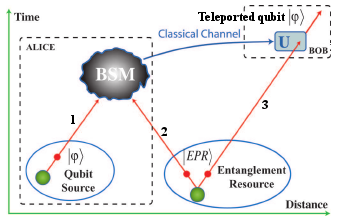
\includegraphics{graphics/Teleportation.png}%
\caption{Schéma de principe de la téléportation quantique. Alice effectue une
mesure de Bell (BSM, Bell State Measurement) sur les qubits $\ket{\psi}$ et un
des qubits EPR et informe Bob du résultat par un canal classique (bits
classiques) afin que ce dernier finalise la téléportation en appliquant une
transformation unitaire $U$ adéquate qui lui permet de reconstruire le qubit
$\ket{\psi}$ envoyé par Alice. [Après N. Gisin and R. Trew, \emph{Quantum
Communication}, \url{http://arxiv.org/abs/quant-ph/0703255v1}]}%
\label{fig:teleportation}%
\end{figure}

Le protocole de téléportation quantique est le suivant:

\begin{itemize}
\item Alice et Bob utilisent un canal EPR composé d'une paire de qubits
maximalement intriqués:
\begin{equation}
\ket{\Phi^{+}}{23}=\frac{1}{\sqrt{2}}(\ket{00}_{23}+\ket{11}_{23}).
\end{equation}
Le qubit $2$ est pris par Alice et le qubit $3$ est pris par Bob.

\item Alice souhaite transmettre ou transférer à Bob l'information sur l'état
d'un qubit
\begin{equation}
\ket{\psi}_{1}=\alpha\ket{0}_{1}+\beta\ket{1} _{1}
\label{eq:Psi1Tel}%
\end{equation}
qui lui est \emph{à priori} inconnu, sans lui transmettre directement ce qubit.

\item Alice mesure l'état quantique de la nouvelle paire de qubits $1$ et $2$
(non intriqués) en utilisant la \textbf{base de Bell} constituée des états
intriquées%
\begin{subequations}%
\label{eq:BellBase}%
\begin{align}
\ket{\Phi^{+}} &  =\frac{1}{\sqrt{2}}(\ket{00}+\ket{11} )\\
\ket{\Phi^{-}} &  =\frac{1}{\sqrt{2}}(\ket{00}-\ket{11} )\\
\ket{\psi^{+}} &  =\frac{1}{\sqrt{2}}(\ket{01}+\ket{10} )\\
\ket{\psi^{-}} &  =\frac{1}{\sqrt{2}}(\ket{01}-\ket{10} ))
\end{align}%
\end{subequations}%
On vérifie facilement que l'état des trois qubits est alors%
\begin{equation}%
\label{eq:Psi123}%
\begin{split}
\ket{\psi}_{123} &  =\ket{\psi}_{1}\otimes\ket{\Phi^{+}}_{23}
=(\alpha\ket{0}+\beta\ket{1})_{1}\otimes\ket{\Phi^{+}}_{23}\\
&  =\frac{1}{2}[\ket{\Phi^{+}}_{12}(\alpha\ket{0}+\beta\ket{1})_{3}+\ket{\Phi
^{-}}_{12}(\alpha\ket{0}-\beta\ket{1})_{3}\\
&  +\ket{\psi^{+}}_{12}(\alpha\ket{1}+\beta\ket{0})_{3}+\ket{\psi^{-}}_{12}
(\alpha\ket{1} -\beta\ket{0})_{3}] \end{split}
\end{equation}%
La mesure par Alice de l'état de la paire de qubits intriqués $12$ projette
cet état sur l'un des quatre états de base (\ref{eq:BellBase}), ce qui
projette l'état du qubit $3$ sur l'état correspondant dans (\ref{eq:Psi123}).
Le tableau \ref{tab:MesBell} récapitule les différentes \emph{mesures de
Bell}:
\begin{table}[htbp]
\centering
\begin{tabular}
[c]{|l|l|l|}\hline\hline
\rowcolor[gray]{0.8}\textbf{Résultat de la mesure de $12$} & \textbf{État
préparé en $3$} & \textbf{probabilité}\\\hline\hline
\multicolumn{1}{|c|}{$\ket{\Phi^{+}}$} &
\multicolumn{1}{|c|}{$\alpha\ket{0}+\beta\ket{1}$} &
\multicolumn{1}{|c|}{$\frac{1}{4}$}\\\hline
\multicolumn{1}{|c|}{$\ket{\Phi^{-}}$} &
\multicolumn{1}{|c|}{$\alpha\ket{0}-\beta\ket{1}$} &
\multicolumn{1}{|c|}{$\frac{1}{4}$}\\\hline
\multicolumn{1}{|c|}{$\ket{\psi^{+}}$} &
\multicolumn{1}{|c|}{$\alpha\ket{0}+\beta\ket{1}$} &
\multicolumn{1}{|c|}{$\frac{1}{4}$}\\\hline
\multicolumn{1}{|c|}{$\ket{\psi^{-}}$} &
\multicolumn{1}{|c|}{$\alpha\ket{0}-\beta\ket{1}$} &
\multicolumn{1}{|c|}{$\frac{1}{4}$}\\\hline
\end{tabular}
\caption{Mesure de Bell qui distingue les quatre états de Bell}
\label{tab:MesBell}%
\end{table}%
On constate que l'état du qubit d'Alice est téléporté sur le qubit de Bob avec
une probabilité de $25\%$.

\item Alice transmet à Bob par un canal classique le résultat de sa mesure
(mesure de Bell), et Bob sait que le qubit $3$ lui arrive dans l'état inconnu
de départ (\ref{eq:Psi1Tel}), mais qui reste tout aussi inconnu! L'état du
qubit $1$ a été téléporté, mais il n'y a jamais eu une mesure de cet état.

\item Si le résultat de la mesure d'Alice n'est pas $\ket{\Phi^{+}}_{12}$, Bob
en sait assez pour faire la correction en appliquant la transformation unitaire
$U$ convenable qui permet de ramener le qubit $3$ dans l'état
(\ref{eq:Psi1Tel}).
\end{itemize}

\begin{remark}
\begin{enumerate}
\item A aucun moment, les coefficients $\alpha$ et $\beta$ ne sont mesurés, et
l'état $\ket{\psi}_{1}$ est détruit au cours de la mesure effectuée pa Alice. Il
n'y a pas contradiction avec le théorème de non-clonage.

\item Bob ne connait l'état du qubit $3$ que lorsqu'il a reçu le résultat de la
mesure d'Alice. La transmission de cette information doit se faire par un canal
classique, à une vitesse au plus égale à la vitesse de la lumière. Il n' a donc
pas transfère instantanée de l'information à distance.

\item Il y a jamais transport de la matière dans la téléportation.
\end{enumerate}
\end{remark}

\newpage

\section{Exercices}

\subsection{QuTiP - Systèmes composites}

On désir étudier un système de deux électrons en interaction. Chaque électron 
est représenté par un sous-système à deux niveaux de base 
$\{\ket{0},\ket{1}\}$. 

Le Hamiltonien du système est
\begin{equation}
\mathtt{H} = \sigma_x\otimes\sigma_z+\mathtt{W}\otimes\mathbb{I},
\end{equation}
où $\sigma_x$ et $\sigma_z$ sont les matrices de Pauli et 
$\mathtt{W}=\dfrac{1}{\sqrt{2}}\begin{pmatrix}1 & 1 \\ 1 & -1 \end{pmatrix}$.

\begin{enumerate}
\item Définir les états $\ket{0}$ et $\ket{1}$.

\item Définir les états de base du système composé des deux électrons en 
interaction.

\item Définir le Hamiltonien du système.

\item Déterminer les valeurs propres et  les vecteurs propres de \texttt{H}.

\item Calculer et normaliser $\ket{\psi}=\mathtt{H}\ket{00}$.
\end{enumerate}

\subsection{QuTiP - Construction d'un état corrélé}

Dans cette exercice, il est question de préparer un état intriqué à partir de 
l'évolution d'un système de deux spins $\frac{1}{2}$.

On considère deux spins $\frac{1}{2}$ dont l'intrication est représentée par le 
Hamiltonien
\begin{equation}
\mathtt{H} = \dfrac{1}{2}\hbar\omega\vec{\sigma_1}\cdot\vec{\sigma_2}.
\end{equation}
Avec, $\sigma_x = \begin{pmatrix}0 & 1 \\ 1 & 0 \end{pmatrix}$, $\sigma_y = 
\begin{pmatrix}0 & -i \\ i & 0 \end{pmatrix}$ et
$\sigma_z = \begin{pmatrix}1 & 0 \\ 0 & -1 \end{pmatrix}$.

La base de calcul est $\{\ket{00},\ket{01},\ket{10},\ket{11}\}$.

\begin{enumerate}
\item Définir le Hamiltonien $\mathtt{H}$ du système ainsi que les états de 
base de calcul.

\item Vérifier pour tous les états de la base de calcul que 
$(\mathbb{I}+\vec{\sigma_1}\cdot\vec{\sigma_2})\ket{ij}=2\ket{ji}$.

\item Déterminer les valeurs propres et les vecteurs propres normalisés du 
Hamiltonien \texttt{H}.

\item On suppose que l'état du système à $t=0$ est $\ket{\psi(0)}=\ket{10}$. 
Résoudre l'équation de shr\"odinger pour $t\in[0,2\pi]$ en utilisant la commande 
\texttt{sesolve(H, Psi0, Temps, [], [])}. Extraire les états $\ket{\psi(t)}$. 
Comparer $\ket{\psi(t=\pi/4)}$ et $\frac{1}{\sqrt{2}}(\ket{10}-i\ket{01})$. 
Pour cela il faut calculer la fidélité : si elle vaut plus de 0.99, on suppose 
que ces deux états sont égaux. La fidélité se calcule à l'aide de la commande 
\texttt{fidelity(Psi1, Psi2)} : elle permet de comparer l'état \texttt{Psi1} à 
l'état \texttt{Psi2}.
\end{enumerate}

\subsection{Inégalités de Bell avec des photons}

On considère deux photons partant en sens inverse, l'un (1) suivant $Oz$ et
l'autre (2) suivant $-Oz$ comme indiqué sur la figure
\ref{fig:ExoInegalitesBell}, dans un état de polarisation intriqué%
\begin{equation}
\ket{\Psi}=\frac{1}{\sqrt{2}}(\ket{xy}-\ket{yx}).
\end{equation}
Les états $\ket{x}$ et $\ket{y}$ sont des états de polarisation linéaire suivant
$Ox$ et $Oy$.

\begin{figure}[ptbh]
\centering
	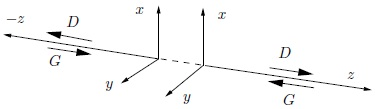
\includegraphics[scale=1]{graphics/ExoInegalitesBell.jpg}
	\caption{Configuration des polarisations des photons intriqués.}
	\label{fig:ExoInegalitesBell}
\end{figure}

\begin{enumerate}
\item L'état de polarisation linéaire suivant la direction $\hat{n}_{\theta}$
du plan $xOy$ est%
\begin{equation}
\ket{\theta}=\cos\theta\ket{x}+\sin\theta\ket{y},
\end{equation}
et l'état de polarisation orthogonale est
\begin{equation}
\ket{\theta_{\bot}}=-\sin\theta\ket{x}+\cos\theta\ket{y}.
\end{equation}
Montrer que%
\begin{equation}
\ket{\Psi}=\frac{1}{\sqrt{2}}(\ket{\theta\theta_{\bot}}-\ket{\theta_{\bot}
\theta}).
\end{equation}
L'état $\ket{\Psi}$ est donc invariant par rotation autour de $Oz$.

\item Montrer que $\ket{\Psi}$ s'écrit, en fonction des états de polarisation
circulaire%
\begin{subequations}
\begin{align}
\ket{D}&  =-\frac{1}{\sqrt{2}}(\ket{x}+i\ket{y}),\\
\ket{G}&  =\frac{1}{\sqrt{2}}(\ket{x}-i\ket{y}),
\end{align}%
\end{subequations}%
en prenant garde au sens de propagation des axes $+Oz$ et $-Oz$ comme indiqué
sur la figure \ref{fig:ExoInegalitesBell},
\begin{equation}
 \ket{\Psi}=\frac{i}{\sqrt{2}}(\ket{DD}-\ket{GG}).
\label{eq:VectDDGG}%
\end{equation}

\item Soient $\mathcal{P}_{D}$ et $\mathcal{P}_{G}$ les projecteurs sur les
états de polarisation circulaire. On peut associer à la grandeur physique
polarisation circulaire l'opérateur
\begin{equation}
\Sigma_{z}=\mathcal{P}_{D}-\mathcal{P}_{G}.
\label{eq:OpPolCirc}%
\end{equation}

\begin{enumerate}
\item Montrer cet opérateur est hermitien et que ses vecteurs propres sont
$\ket{D}$ et $\ket{G}$.

\item En utilisant (\ref{eq:OpPolCirc}), vérifier que (\ref{eq:VectDDGG}) est
invariant par rotation autour de $Oz$.
\end{enumerate}

\item Alice et Bob analysent la polarisation des photons à l'aide de
polariseurs linéaires orientés suivant les directions $\hat{n}_{\alpha}$ pour
le photon 1 et $\hat{n}_{\beta}$ pour le photon 2 dans le plan $xOy$. On définit

\begin{itemize}
\item $\texttt{p}{++}(\alpha,\beta)$, la probabilité pour que le photon 1 soit
polarisé suivant $\hat{n}_{\alpha}$ et le photon 2 suivant $\hat{n}_{\beta}$;

\item $\texttt{p}_{+-}(\alpha,\beta)$, la probabilité pour que le photon 1 soit
polarisé suivant $\hat{n}_{\alpha}$ et le photon 2 suivant
$\hat{n}_{\beta_{\bot}}$;

\item $\texttt{p}_{-+}(\alpha,\beta)$ et $\texttt{p}_{--}(\alpha,\beta)$ étant
définis de façon analogue.
\end{itemize}

On définit le coefficient de corrélation de polarisation%
\begin{equation}
E(\alpha,\beta)=[\texttt{p}_{++}(\alpha,\beta)+\texttt{p}_{--}(\alpha,\beta)]-[
\texttt{p}_{+-} (\alpha,\beta) +\texttt{p}_{+-}(\alpha,\beta)].
\end{equation}


\begin{enumerate}
\item En utilisant l'invariant par rotation de $\ket{\Psi}$ pour simplifier
les calculs, trouver l'expression des probabilités précédentes et montrer que%
\begin{equation}
E(\alpha,\beta)=-\cos[-2(\alpha-\beta)].
\end{equation}

\item Quelles valeurs de $\alpha$, $\alpha^{\prime}$, $\beta$ et
$\beta^{\prime}$ doit-on utiliser pour obtenir comme dans le cas des spins
$\frac{1}{2}$,
\begin{equation}
X=E(\alpha,\beta)+E(\alpha,\beta^{\prime})+E(\alpha^{\prime},\beta^{\prime
})-E(\alpha^{\prime},\beta)=-2\sqrt{2}?
\end{equation}

\end{enumerate}

\item Montrer que
\begin{equation}
\ket{\Phi}=\frac{1}{\sqrt{2}}(\ket{xx}+\ket{yy}),
\end{equation}
est également invariant par rotation autour de $Oz$. Donner son expression en
fonction des états de polarisation circulaire.
\end{enumerate}


\subsection{Distribution quantique des clefs 1}

\subsubsection{BB4 sans espion}

\begin{enumerate}
\item Compléter le tableau \ref{tab:BB4SSEspion} qui décrit la phase
\textbf{Envoie}.

\item Vérifier qu'après la phase \textbf{sifting}, Alice et Bob partagent une
liste identique de bits secrets. Pourquoi ces bits sont-ils secrets?
\end{enumerate}

\begin{table}[ptbh]
\centering
{\footnotesize {
\begin{tabular}
[c]{|l|l|l||l|l|l|}\hline
\rowcolor[gray]{0.8}\textbf{A envoie} & \textbf{B mesure et trouve} &
\textbf{Probabilité} & \textbf{A envoie} & \textbf{B mesure et trouve} &
\textbf{Probabilité}\\\hline
\multicolumn{1}{|c|}{$\ket{0_{z}}$} &
\multicolumn{1}{|c|}{$Z\rightarrow\ket{0_{z}}$} &
\multicolumn{1}{|c||}{$1$} & \multicolumn{1}{||c|}{$\ket{0_{x}}$} &
\multicolumn{1}{|c|}{$Z\rightarrow\ket{0_{z}}$} &
\multicolumn{1}{|c|}{}\\\hline
\multicolumn{1}{|c|}{$\ket{0_{z}}$} &
\multicolumn{1}{|c|}{$Z\rightarrow\ket{1_{z}}$} &
\multicolumn{1}{|c||}{} & \multicolumn{1}{||c|}{$\ket{0_{x}}
$} & \multicolumn{1}{|c|}{$Z\rightarrow\ket{1_{z}}$} &
\multicolumn{1}{|c|}{}\\\hline
\multicolumn{1}{|c|}{$\ket{0_{z}}$} &
\multicolumn{1}{|c|}{$X\rightarrow\ket{0_{x}}$} &
\multicolumn{1}{|c||}{$\frac{1}{2}$} & \multicolumn{1}{||c|}{$\ket{0_{x}}$} &
\multicolumn{1}{|c|}{$X\rightarrow\ket{0_{x}}$} & \multicolumn{1}{|c|}{}\\\hline
\multicolumn{1}{|c|}{$\ket{0_{z}}$} &
\multicolumn{1}{|c|}{$X\rightarrow\ket{1_{x}}$} &
\multicolumn{1}{|c||}{} & \multicolumn{1}{||c|}{$\ket{0_{x}}
$} & \multicolumn{1}{|c|}{$X\rightarrow\ket{1_{x}}$} &
\multicolumn{1}{|c|}{}\\\hline\hline
\multicolumn{1}{|c|}{$\ket{1_{z}}$} &
\multicolumn{1}{|c|}{$Z\rightarrow\ket{0_{z}}$} &
\multicolumn{1}{|c||}{} & \multicolumn{1}{||c|}{$\ket{1_{x}}
$} & \multicolumn{1}{|c|}{$Z\rightarrow\ket{0_{z}}$} &
\multicolumn{1}{|c|}{}\\\hline
\multicolumn{1}{|c|}{$\ket{1_{z}}$} &
\multicolumn{1}{|c|}{$Z\rightarrow\ket{1_{z}}$} &
\multicolumn{1}{|c||}{} & \multicolumn{1}{||c|}{$\ket{1_{x}}
$} & \multicolumn{1}{|c|}{$Z\rightarrow\ket{1_{z}}$} &
\multicolumn{1}{|c|}{}\\\hline
\multicolumn{1}{|c|}{$\ket{1_{z}}$} &
\multicolumn{1}{|c|}{$X\rightarrow\ket{0_{x}}$} &
\multicolumn{1}{|c||}{} & \multicolumn{1}{||c|}{$\ket{1_{x}}
$} & \multicolumn{1}{|c|}{$X\rightarrow\ket{0_{x}}$} &
\multicolumn{1}{|c|}{}\\\hline
\multicolumn{1}{|c|}{$\ket{1_{z}}$} &
\multicolumn{1}{|c|}{$X\rightarrow\ket{1_{x}}$} &
\multicolumn{1}{|c||}{} & \multicolumn{1}{||c|}{$\ket{1_{x}}
$} & \multicolumn{1}{|c|}{$X\rightarrow\ket{1_{x}}$} &
\multicolumn{1}{|c|}{}\\\hline
\end{tabular}
}}\caption{Phase \textbf{envoie} d'une situation idéale sans espion ni erreurs
du protocole BB84 sans espion}%
\label{tab:BB4SSEspion}%
\end{table}

\subsubsection{BB4 avec espion}

On suppose qu'une espionne Eve (E) fait la même chose que Bob, en choisissant
de mesurer soit $Z$ soit $X$ . Ensuite, elle prépare un nouveau photon
polarisé suivant le résultat de sa mesure qu'elle envoie à Bob. On appelle
cette attaque \textbf{intercept-resend}.

Pour le tableau \ref{tab:BB4AVEspion} de la phase \textbf{Envoie}, nous ne
considérons que les cas où Alice et Bob mesurent dans la même base, car les
autres cas seront de toute façon écartés lors de la phase \textbf{sifting}.
Aussi nous ne considérons que la base $Z$, la situation pour la base $X$ étant
symétrique.

\begin{enumerate}
\item Compléter les probabilités du tableau \ref{tab:BB4AVEspion}. On notera
qu'Alice et Bob n'ont pas le même bit en présence de l'attaque d'Eve, malgré
le fait qu'ils ont effectué les mesures dans la même base.

\item Pourquoi dans le protocole BB4 est-il nécessaire d'utiliser deux bases?
Que se passerait-il si Alice et Bob décidaient de n'utiliser qu'une seule base
pour coder leurs bits?

\item Comment Alice et Bob font pour détecter la présence de l'espion Eve?
\end{enumerate}

\begin{table}[ptbh]
\centering
{\footnotesize {
\begin{tabular}
[c]{|l|p{2cm}|p{2.1cm}|l|l|p{2cm}|p{2.1cm}|l|}\hline
\rowcolor[gray]{0.8}\textbf{A envoie} & \textbf{E mesure et trouve} &
\textbf{B mesure et trouve} & \textbf{Proba} &
\textbf{A envoie} & \textbf{E mesure et trouve} &
\textbf{B mesure et trouve} & \textbf{Probab}\\\hline
\multicolumn{1}{|c|}{$\ket{0_{z}}$} &
\multicolumn{1}{|c|}{$Z\rightarrow\ket{0_{z}}$} &
\multicolumn{1}{|c|}{$Z\rightarrow\ket{0_{z}}$} &
\multicolumn{1}{|c|}{$\frac{1}{2}$} & \multicolumn{1}{|c|}{$\ket{1_{z}}$} &
\multicolumn{1}{|c|}{$Z\rightarrow\ket{0_{z}}$} &
\multicolumn{1}{|c|}{$Z\rightarrow\ket{0_{z}}$} & \multicolumn{1}{|c|}{}\\\hline
\multicolumn{1}{|c|}{$\ket{0_{z}}$} &
\multicolumn{1}{|c|}{$Z\rightarrow\ket{0_{z}}$} &
\multicolumn{1}{|c|}{$Z\rightarrow\ket{1_{z}}$} &
\multicolumn{1}{|c|}{$0$} & \multicolumn{1}{|c|}{$\ket{1_{z}}$} &
\multicolumn{1}{|c|}{$Z\rightarrow\ket{0_{z}}$} &
\multicolumn{1}{|c|}{$Z\rightarrow\ket{1_{z}}$} &
\multicolumn{1}{|c|}{}\\\hline
\multicolumn{1}{|c|}{$\ket{0_{z}}$} &
\multicolumn{1}{|c|}{$Z\rightarrow\ket{1_{z}}$} &
\multicolumn{1}{|c|}{$Z\rightarrow\ket{0_{z}}$} &
\multicolumn{1}{|c|}{} & \multicolumn{1}{|c|}{$\ket{1_{z}}
$} & \multicolumn{1}{|c|}{$Z\rightarrow\ket{1_{z}}$} &
\multicolumn{1}{|c|}{$Z\rightarrow\ket{0_{z}}$} &
\multicolumn{1}{|c|}{}\\\hline
\multicolumn{1}{|c|}{$\ket{0_{z}}$} &
\multicolumn{1}{|c|}{$Z\rightarrow\ket{1_{z}}$} &
\multicolumn{1}{|c|}{$Z\rightarrow\ket{1_{z}}$} &
\multicolumn{1}{|c|}{} & \multicolumn{1}{|c|}{$\ket{1_{z}}
$} & \multicolumn{1}{|c|}{$Z\rightarrow\ket{1_{z}}$} &
\multicolumn{1}{|c|}{$Z\rightarrow\ket{1_{z}}$} &
\multicolumn{1}{|c|}{}\\\hline
\multicolumn{1}{|c|}{$\ket{0_{z}}$} &
\multicolumn{1}{|c|}{$X\rightarrow\ket{0_{x}}$} &
\multicolumn{1}{|c|}{$Z\rightarrow\ket{0_{z}}$} &
\multicolumn{1}{|c|}{$\frac{1}{8}$} & \multicolumn{1}{|c|}{$\ket{1_{z}}$} &
\multicolumn{1}{|c|}{$X\rightarrow\ket{0_{x}}$} &
\multicolumn{1}{|c|}{$Z\rightarrow\ket{0_{z}}$} & \multicolumn{1}{|c|}{}\\\hline
\multicolumn{1}{|c|}{$\ket{0_{z}}$} &
\multicolumn{1}{|c|}{$X\rightarrow\ket{0_{x}}$} &
\multicolumn{1}{|c|}{$Z\rightarrow\ket{1_{z}}$} &
\multicolumn{1}{|c|}{} & \multicolumn{1}{|c|}{$\ket{1_{z}}
$} & \multicolumn{1}{|c|}{$X\rightarrow\ket{0_{x}}$} &
\multicolumn{1}{|c|}{$Z\rightarrow\ket{1_{z}}$} &
\multicolumn{1}{|c|}{}\\\hline
\multicolumn{1}{|c|}{$\ket{0_{z}}$} &
\multicolumn{1}{|c|}{$X\rightarrow\ket{1_{x}}$} &
\multicolumn{1}{|c|}{$Z\rightarrow\ket{0_{z}}$} &
\multicolumn{1}{|c|}{} & \multicolumn{1}{|c|}{$\ket{1_{z}}
$} & \multicolumn{1}{|c|}{$X\rightarrow\ket{1_{x}}$} &
\multicolumn{1}{|c|}{$Z\rightarrow\ket{0_{z}}$} &
\multicolumn{1}{|c|}{}\\\hline
\multicolumn{1}{|c|}{$\ket{0_{z}}$} &
\multicolumn{1}{|c|}{$X\rightarrow\ket{1_{x}}$} &
\multicolumn{1}{|c|}{$Z\rightarrow\ket{1_{z}}$} &
\multicolumn{1}{|c|}{} & \multicolumn{1}{|c|}{$\ket{1_{z}}
$} & \multicolumn{1}{|c|}{$X\rightarrow\ket{1_{x}}$} &
\multicolumn{1}{|c|}{$Z\rightarrow\ket{1_{z}}$} &
\multicolumn{1}{|c|}{}\\\hline
\end{tabular}
}}
\caption{Phase \textbf{envoie} d'une situation avec espion du protocole BB84}%
\label{tab:BB4AVEspion}%
\end{table}

\subsection{Distribution quantique des clefs 1}

\emph{\small Deux personnes qui veulent communiquer dans l'intimité ou la
discrétion doivent prévoir une clef et la garder sécrète. Le code de Vernam est
le seul qui soit mathématiquement reconnu comme inviolable, mais il impose
d'utiliser une clef différente pour chaque chiffrement. C'est problème de
distribution des clefs secrètes. Le présent exercice montre comment la théorie
quantique peut fournir une procédure répondant à ce besoin.}

 On rappelle que $\cos^4x+\sin^4x=\frac{1}{2}(1+\cos^22x)$ et
$\int(1+\cos^2x)dx= \frac{3}{2}x+\frac{1}{4}\sin2x$.
\begin{enumerate}
\item On considère un quanton de spin $\frac{1}{2}$. L'opérateur de spin est
$\bls{S}=\frac{\hbar}{2}\bls{\sigma}$, où les $\bls{\sigma}$
sont les matrices de Pauli,
qui dans la base $\{\ket{z+},\ket{z-}\}$ qui diagonalise $\mathtt{S}_z$
s'écrivent,
\begin{equation}
\sigma_x=\ket{z-}\bra{z+}+\ket{z+}\bra{z-},\,\sigma_y=i(\ket{z-}\bra{z+}
-\ket{z+}\bra{z-}),\,\sigma_z=\ket{z+}\bra{z+}-\ket{z-}\bra{z-}.
\end{equation}
On suppose que l'état du spin du quanton est $\ket{z+}$. On effectue la mesure
de la composante du spin suivant un axe orienté le long du vecteur unitaire
$\bls{\hat{u}}(\sin\theta,0,\cos\theta)$. Les états propre de
$\mathtt{S}_u$,
$\ket{u+}$ et $\ket{u-}$ sont les transformés des états $\ket{z\pm}$ par une
rotation qui amène l'axe $Oz$ sur l'axe $\bls{\hat{u}}$. Un choix possible
consiste à faire une rotation de $\theta$ autour de l'axe $Oy$. On rappelle que
l'opérateur de rotation autour de $Ou$ est $\mathtt{R}_u(\theta)=
e^{-i\theta\sigma_{u}/2} =(\cos\frac{\theta}{2})\mathbb{I}
-i(\sin\frac{\theta}{2})\sigma_{u}$.

\begin{enumerate}
 \item Donner l'expression de $\ket{u\pm}$ en fonction de $\theta$. En déduire
les probabilités $\mathcal{P}^{\pm}_{u\leftarrow z+}(\theta)$ de trouver
$\pm\frac{\hbar}{2}$
suivant $u$, l'état mesuré étant $\ket{z+}$.

\item Quels sont les états de spins après une mesure ayant donné
$+\frac{\hbar}{2}$ ou $-\frac{\hbar}{2}$?
\end{enumerate}

\item Immédiatement après cette mesure, on mesure la composante du spin suivant
l'axe $z$.

\begin{enumerate}
 \item Donner les résultats possibles  et leurs probabilités en fonction du
résultat obtenu précédemment le long de $u$.

\item Montrer que la probabilité de retrouver la même valeur $+\frac{\hbar}{2}$
que dans l'état initial $\ket{z+}$ est,
\begin{equation}
  \mathcal{P}_{++}(\theta)=\frac{1}{2}(1+\cos^2\theta).
\end{equation}

\item En supposant, maintenant que l'état initial soit $\ket{z-}$, quelle est,
dans la même séquence de mesures, la probabilité $\mathcal{P}_{--}(\theta)$ de
retrouver $-\frac{\hbar}{2}$ dans la dernière mesure? On se contentera d'une
brève justification!
\end{enumerate}

\item On dispose d'une source $O$ qui produit une paire $(a,b)$ de quantons de
spins $\frac{1}{2}$, préparé dans l'état $\ket{\psi}=\phi(\bls{r}_a,\bls{r}_b)
\ket{\Sigma}$ où l'état du spin des 2 quantons est
\begin{equation}
 \ket{\Sigma}=\frac{1}{\sqrt{2}}(\ket{z+}\ket{z+}+\ket{z-}\ket{z-})
 =\frac{1}{\sqrt{2}}(\ket{z+z+}+\ket{z-z-}),\label{eq:Sigma1}
\end{equation}
c'est-à-dire que les variables spatiales et les variables de spin sont
indépendantes. Dans la suite, on ne s'intéresse qu'aux mesures du spin.

\begin{enumerate}
 \item Montrer que l'état (\ref{eq:Sigma1}) peut également s'écrire
 \begin{equation}
 \ket{\Sigma}=\frac{1}{\sqrt{2}}(\ket{x+x+}+\ket{x-x-}).\label{eq:Sigma2}
\end{equation}

\item La paire de quanton $(a,b)$ étant préparé dans l'état (\ref{eq:Sigma1}) ou
(\ref{eq:Sigma2}), ces quanton sont spatialement séparés (voir la figure
\ref{fig:PaireAB}) sans que l'état de spin ne soit affecté (avant qu'une mesure
n'intervienne).

\begin{figure}[htbp]
 \centering
 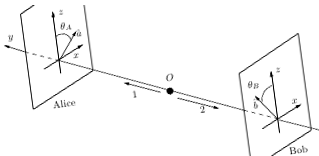
\includegraphics[scale=1]{./graphics/ExoPaireAB.png}
 \caption{Configuration des axes pour l'expérience de mesure de deux spins.}
 \label{fig:PaireAB}
\end{figure}

\begin{enumerate}
 \item Alice mesure d'abord la composante du spin de $a$ suivant un axe $u_a$
d'angle $\theta_a$. Quels sont les résultats de mesure et les probabilités
correspondantes dans les deux cas $\theta_a=0$ (z) et $\theta_a=\frac{\pi}{2}$
(x)?

\item Après cette mesure d'Alice l'état de spin des deux quantons est
\begin{center}
\begin{tabular}{|c|c|c|}\hline
Axe & Résultat & État\\\hline
$z$ & $+\frac{\hbar}{2}$ & $\ket{z+z+}$\\\hline
$z$ & $-\frac{\hbar}{2}$ & $\ket{z-z-}$\\\hline
$x$ & $+\frac{\hbar}{2}$ & $\ket{x+x+}$\\\hline
$x$ & $-\frac{\hbar}{2}$ & $\ket{x-x-}$\\\hline
 \end{tabular}
 \end{center}
En déduire qu'on peut désormais ignorer le quanton $a$ pour ce qui concerne les
mesures de spin sur $b$.
\end{enumerate}

\item Après cette mesure d'Alice, Bob mesure la composante du spin de $b$
suivant un axe $u_b$ d'angle $\theta_b$. Déterminer les résultats de
mesure possible de Bob et leurs probabilités, en fonction du résultat d'Alice,
dans les quatre configurations suivantes:
\begin{center}
\begin{tabular}{|c|c|c|c|}\hline
$(\theta_a,\theta_b)$ & Résultat Alice & Résultat Bob & Probabilité\\\hline
$(0,0)$ &  & &\\\hline
$(0,\frac{\pi}{2})$ &  & &\\\hline
$(\frac{\pi}{2},0)$ &  & &\\\hline
$(\frac{\pi}{2},\frac{\pi}{2})$ &  & &\\\hline
 \end{tabular}
 \end{center}
Dans quel(s) cas la mesure sur $a$ et celle sur $b$ donnent-elles certainement 
le même résultat?

\item On se place dans la situation $\theta_a=0$. On suppose qu'un
\emph{espion}, situé entre la source $O$ et Bob, fait une mesure de la
composante du spin $b$ suivant un axe $u_e$ d'angle $\theta_e$.

\begin{enumerate}
 \item Quels sont, en fonction de $\theta_e$ et du résultat de mesure d'Alice,
les résultats de mesure de l'espion et leurs probabilités?

\item Après cette mesure de l'espion, Bob mesure le spin de $b$ suivant l'axe
défini par $\theta_b=0$, que trouve-t-il, avec quelle probabilité, en fonction
du résultat trouvé par l'espion?

\item Quelle est la probabilité $\mathcal{P}(\theta_e)$ qu'Alice et Bob
trouvent le même résultat?

\item Quelle est la moyenne de $\mathcal{P}(\theta_e)$ si l'espion
 choisit au hasard $\theta_e$ avec une probabilité uniforme sur $[0,2\pi]$
($\frac{1}{2\pi}\int_0^{2\pi}\mathcal{P}(\theta_e)d\theta_e$)? Quelle est cette
même moyenne s'il choisit équitablement seulement les deux valeurs
$\theta_e=0$, et $\theta_e=\frac{\pi}{2}$?
\end{enumerate}
\end{enumerate}

\item On souhaite utiliser les résultats qui précèdent à la transmission
confidentielle d'information. Alice et Bob utilisent alors la procédure
ci-dessous:
{\small
\begin{itemize}
 \item Alice et Bob décident d'un choix d'axes $x$ et $z$ qui leurs servent de
direction d'analyse.

\item Alice, qui dispose de la source $O$ prépare une séquence ordonnée de
$N\gg n$ paires de spins $\frac{1}{2}$ dans l'état (\ref{eq:Sigma1}) ($n$ est
le nombre de bits du message). Elle envoie les spins $b$ à Bob, et garde les
spins $a$.

\item Alice et Bob font, pour chacun des spins dont ils disposent, la mesure de
la composante $x$ ou $z$. Le choix entre $x$ et $z$ se fait de manière
aléatoire et équiprobable pour chaque spin, et il n'y a pas de corrélation,
pour un spin donné, entre la composante choisie par Alice et celle choisie par
Bob. Ils stockent chacun l'ensemble de leurs résultats.

\item Bob sélectionne une partie $FN$ de ses mesures et il les communique
publiquement à Alice, par un canal classique, la direction d'analyse choisie et
le résultat obtenu pour chacune des mesures de cet ensemble. En pratique
$F\sim0.5$.

\item Alice compare pour cet ensemble $FN$ ses directions et ses résultats avec
ceux que vient de lui communiquer Bob. Elle peut alors détecter la présence
éventuelle d'un espion. Si un espion est repéré, la procédure s'arrête et une
recherche \emph{physique} de l'espion doit avoir lieu. Sinon,

\item Alice annonce publiquement qu'elle est convaincue de ne pas avoir été
écoutée, et Bob lui transmet, toujours publiquement, ses directions d'analyse
pour les $(1-F)N$ spins restants. En revanche, il ne communique pas ses
résultats correspondants.
\end{itemize}
}

\begin{enumerate}
 \item Comment Alice peut-elle se convaincre de la présence d'un espion dans le
cas idéal des détecteurs parfaits?

 \item Quelle est la probabilité qu'un espion présent ne soit pas détecté?
A.N.: $FN=200$.

\item L'espion gagne-t-il en \emph{invisibilité} s'il connaît le système d'axe
$Oxz$ retenu par Alice et Bob et déterminant les directions d'analyse?

\item Discuter sur les deux expériences décrites ci-dessous par les tables
\ref{tab:Exp1} et \ref{tab:Exp2}, l'existence d'un espion. On montrera que la
communication 2 a certainement été espionnée. On calculera la probabilité qu'un
espion ait opéré sans être détecté dans la communication 1.

\item Donner la dernière phase de la procédure en indiquant comment Alice peut
envoyer son message (1) à Bob, sans utiliser d'autres paires de spins que les
$N$ paires déjà produites et analyser par Bob et elle-même. En utilisant les
colonne grisées de la table \ref{tab:Exp1}, indiquer comment dans l'expérience 1
ci-dessus, Alice peut transmettre à Bob le message $\{+,-\}$.
\end{enumerate}

\end{enumerate}

\begin{table}[htp]
\centering
\begin{tabular}{|l|c|c|c|c|c|c|c|c|c|c|c|c|}\hline
Numéro Spin & 1 &\cellcolor[gray]{.8} 2 & 3 & 4 &\cellcolor[gray]{.8} 5
&\cellcolor[gray]{.8} 6 & 7 &\cellcolor[gray]{.8} 8 &\cellcolor[gray]{.8} 9 & 10
& 11 &\cellcolor[gray]{.8} 12\\\hline
Axe  choisi par Alice (secret) & X &\cellcolor[gray]{.8} X & Z & X
&\cellcolor[gray]{.8} Z &\cellcolor[gray]{.8} Z & X &\cellcolor[gray]{.8} Z
&\cellcolor[gray]{.8} Z & Z & X &\cellcolor[gray]{.8}
X\\\hline
Résultat d'Alice (secret) & + &\cellcolor[gray]{.8} - & + & +
&\cellcolor[gray]{.8} - &\cellcolor[gray]{.8} - & + &\cellcolor[gray]{.8} +
&\cellcolor[gray]{.8} + & - & + &\cellcolor[gray]{.8}
-\\\hline
Axe choisi par Bob (publique) & X &  & X & Z &  &  & X &  &  & X & X &
\\\hline
Résultat de Bob (publique) & + &  & - & - &  &  & + &  &  & + & + & \\\hline
\end{tabular}
\caption{\small Expérience 1 réalisée avec $N=12$ paires de spins.}
\label{tab:Exp1}
\end{table}

\begin{table}[htp]
\centering
\begin{tabular}{|l|c|c|c|c|c|c|c|c|c|c|c|c|}\hline
Numéro Spin & 1 & 2 & 3 & 4 & 5 & 6 & 7 & 8 & 9 & 10 & 11 &  12\\\hline
Axe  choisi par Alice (secret) & X & Z & Z & Z & X & X & Z & X & X & Z & X &
Z\\\hline
Résultat d'Alice (secret) & + & + & - & + & + & - & + & + & - & - & + &
+\\\hline
Axe choisi par Bob (publique) &  & X &  &  & X &  &  & X & Z &  & Z & Z\\\hline
Résultat de Bob (publique) &  &  +&  &  & + &  & & - & + & +& + & -\\\hline
\end{tabular}
\caption{\small Expérience 2 réalisée avec $N=12$ paires de spins.}
\label{tab:Exp2}
\end{table}

